\documentclass[./main.tex]{subfiles}
\graphicspath{{\subfix{./figs}}}

% ------------ main document ------------ 
\begin{document}
\chapter{\chapEco} \label{chap:ecoeco}

% custom paragraph skip
\setlength{\parskip}{0mm}

\epigraph{\small{Quando trabalhei no Banco Mundial, frequentemente ouvia a afirmação: \say{Não há conflito entre economia e ecologia. Podemos e devemos fazer a economia crescer e proteger o meio ambiente ao mesmo tempo}. Ainda ouço isso com frequência hoje em dia.}}{Herman Daly (2015, p. 1) \cite{Daly2015a}}

\epigraph{\small{Lorem ipsum dolor sit amet consectetur adipiscing elit. Sed ac bibendum orci. Cras erat elit, consequat vel erat ac, tincidunt pulvinar lacus. Pellentesque vitae consectetur quam. Interdum et malesuada fames ac ante ipsum primis in faucibus.}}{Name (Year, p. n) [>>cite]}

% custom paragraph skip
\setlength{\parskip}{\myparskip}

\section{SecIntro} \label{chap:ecoeco:sec1}

\par Cras erat elit, consequat vel erat ac, tincidunt pulvinar lacus. Pellentesque vitae consectetur quam. Interdum et malesuada fames ac ante ipsum primis in faucibus. Curabitur at mollis eros. Integer ornare erat neque, id finibus velit ultrices in. Suspendisse dapibus tortor eget lorem pretium venenatis. Cras erat elit, consequat vel erat ac, tincidunt pulvinar lacus. Pellentesque vitae consectetur quam. Interdum et malesuada fames ac ante ipsum primis in faucibus. Curabitur at mollis eros. Integer ornare erat neque, id finibus velit ultrices in. Suspendisse dapibus tortor eget lorem pretium venenatis. Cras erat elit, consequat vel erat ac, tincidunt pulvinar lacus. Pellentesque vitae consectetur quam. Interdum et malesuada fames ac ante ipsum primis in faucibus. Curabitur at mollis eros. Integer ornare erat neque, id finibus velit ultrices in. Suspendisse dapibus tortor eget lorem pretium venenatis.

\begin{figure}[t!] 
\centering				
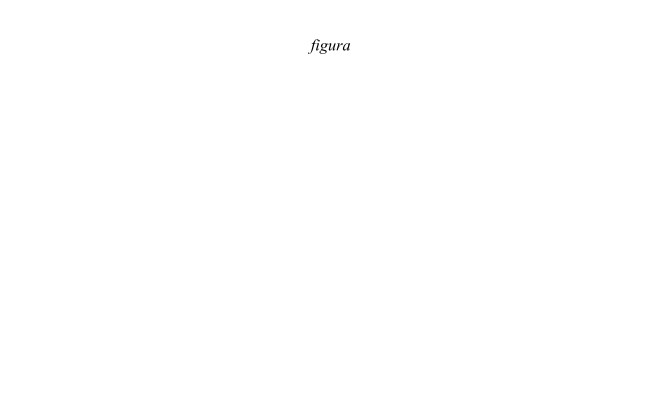
\includegraphics[width=0.98\linewidth]{figs/fig_m.jpg}		
\caption[Lorem ipsum dolor sit amet]
{\textbf{---\;Lorem ipsum dolor sit amet.}
    Lorem ipsum dolor sit amet consectetur adipiscing elit. Sed ac bibendum orci. Cras erat elit, consequat vel erat ac, tincidunt pulvinar lacus. \;\textbf{a}\;---\;Sed ac bibendum orci. Cras erat elit, consequat vel erat ac, tincidunt pulvinar lacus. Pellentesque vitae consectetur quam. Interdum et malesuada fames ac ante ipsum primis in faucibus.\;\textbf{b}\;---\;Sed ac bibendum orci. Cras erat elit, consequat vel erat ac, tincidunt pulvinar lacus. Pellentesque vitae consectetur quam. Interdum et malesuada fames ac ante ipsum primis in faucibus. \;\textbf{c}\;---\;Sed ac bibendum orci. Cras erat elit, consequat vel erat ac, tincidunt pulvinar lacus. Pellentesque vitae consectetur quam. Interdum et malesuada fames ac ante ipsum primis in faucibus.
}
\label{fig:eco:intro} 		
\end{figure}

\par Cras erat elit, consequat vel erat ac, tincidunt pulvinar lacus. Pellentesque vitae consectetur quam. Interdum et malesuada fames ac ante ipsum primis in faucibus. Curabitur at mollis eros. Integer ornare erat neque, id finibus velit ultrices in. Suspendisse dapibus tortor eget lorem pretium venenatis. Cras erat elit, consequat vel erat ac, tincidunt pulvinar lacus. Pellentesque vitae consectetur quam. Interdum et malesuada fames ac ante ipsum primis in faucibus. Curabitur at mollis eros. Integer ornare erat neque, id finibus velit ultrices in. Suspendisse dapibus tortor eget lorem pretium venenatis. Cras erat elit, consequat vel erat ac, tincidunt pulvinar lacus. Pellentesque vitae consectetur quam. Interdum et malesuada fames ac ante ipsum primis in faucibus. Curabitur at mollis eros. Integer ornare erat neque, id finibus velit ultrices in. Suspendisse dapibus tortor eget lorem pretium venenatis.

\par Cras erat elit, consequat vel erat ac, tincidunt pulvinar lacus. Pellentesque vitae consectetur quam. Interdum et malesuada fames ac ante ipsum primis in faucibus. Curabitur at mollis eros. Integer ornare erat neque, id finibus velit ultrices in. Suspendisse dapibus tortor eget lorem pretium venenatis. Cras erat elit, consequat vel erat ac, tincidunt pulvinar lacus. Pellentesque vitae consectetur quam. Interdum et malesuada fames ac ante ipsum primis in faucibus. Curabitur at mollis eros. Integer ornare erat neque, id finibus velit ultrices in. Suspendisse dapibus tortor eget lorem pretium venenatis. Cras erat elit, consequat vel erat ac, tincidunt pulvinar lacus. Pellentesque vitae consectetur quam. Interdum et malesuada fames ac ante ipsum primis in faucibus. Curabitur at mollis eros. Integer ornare erat neque, id finibus velit ultrices in. Suspendisse dapibus tortor eget lorem pretium venenatis.

\par Antes de se examinar o emprego de modelos hidrológicos no planejamento de políticas de conservação ou revitalização de bacias hidrográficas, precisarei aqui fazer uma digressão, de forma a se estabelecer fundamentos teóricos sólidos sobre o que significam os populares termos\say{desenvolvimento sustentável} ou \say{serviços ambientais}. Tentarei ser breve, mas o assunto é extenso e tomado por muitos jargões e definições, além de apresentar um histórico muito rico do pensamento econômico do último século. 

\section{Fins e meios: Economia} \label{chap:ecoeco:economy}

\begin{figure}[t!] 
\centering				
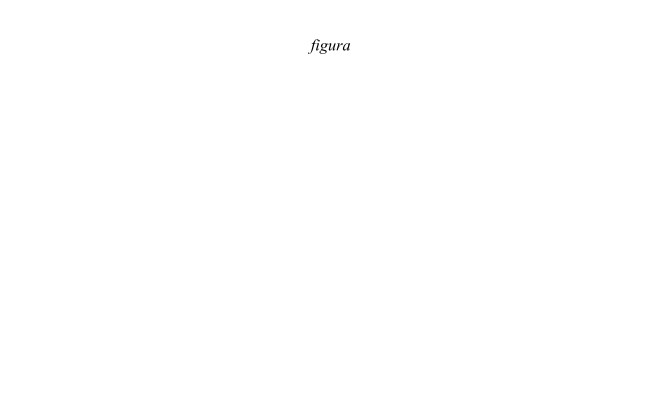
\includegraphics[width=0.98\linewidth]{figs/fig_m.jpg}		
\caption[O espectro da Economia]
{\textbf{---\;O espectro da \gls{gseconomics}.}
    Lorem ipsum dolor sit amet consectetur adipiscing elit. Sed ac bibendum orci. Cras erat elit, consequat vel erat ac, tincidunt pulvinar lacus. \;\textbf{a}\;---\;Sed ac bibendum orci. Cras erat elit, consequat vel erat ac, tincidunt pulvinar lacus. Pellentesque vitae consectetur quam. Interdum et malesuada fames ac ante ipsum primis in faucibus.\;\textbf{b}\;---\;Sed ac bibendum orci. Cras erat elit, consequat vel erat ac, tincidunt pulvinar lacus. Pellentesque vitae consectetur quam. Interdum et malesuada fames ac ante ipsum primis in faucibus. \;\textbf{c}\;---\;Sed ac bibendum orci. Cras erat elit, consequat vel erat ac, tincidunt pulvinar lacus. Pellentesque vitae consectetur quam. Interdum et malesuada fames ac ante ipsum primis in faucibus.
}
\label{fig:eco:economy} 		
\end{figure}

\par A \textbf{\gls{gseconomics}} é a ciência que se dedica ao estudo da alocação de recursos escassos entre diferentes objetivos. Por exemplo, podemos optar por utilizar aço na construção de casas ou de mísseis; destinar água para irrigação agrícola ou geração de energia; usar a terra para manter florestas tropicais de pé ou para criar e abater vacas. Qual é a melhor opção? Se os recursos citados são realmente escassos, essas opções não são meras falsas dicotomias falaciosas, mas questões muito sérias, com consequências drasticamente diferentes entre uma escolha e a outra. Nesse sentido, a \gls{gseconomics} não está somente associada à existência de recursos escassos, mas também está intrinsecamente ligada ao processo de tomada de \textbf{decisões}, de fazer escolhas, pois não se pode ter tudo ao mesmo tempo. Disso, a seguinte pergunta central se impõe:

-- Quais são os objetivos que guiam as escolhas?

\noindent Esta claramente não é uma pergunta empírica. Ela não pode ser respondida fazendo-se uma expedição de campo e testando hipóteses contra as evidências observadas, como são as perguntas sobre problemas científicos. Nesse caso, o mundo empírico simplesmente ofereceria uma confusão de respostas contraditórias. Tampouco é uma pergunta Lógica, que pode ser respondida a partir de axiomas fundamentais, como na Geometria. A pergunta revela-se, portanto, essencialmente \textbf{\gls{gsethics}}: ela pressupõe um valor moral daquilo que \textit{deve} ser objetivado\footnote{Esse tipo que questão também denomina-se \textbf{normativa}.}. A \gls{gsethics} é o ramo da Filosofia que explora os princípios e valores que orientam o comportamento humano, buscando definir o que é considerado certo ou errado, justo ou injusto, o que deve ser feito e aquilo que não deve ser feito. Por isso, a pergunta central da \gls{gseconomics} depende de uma orientação \gls{gsethics}. 

\par No âmbito estrito da Biologia, é claro, todos os organismos precisam lidar com a alocação de recursos escassos para endereçar o \textbf{\gls{existimper}}, que não tem nada a ver com \gls{gsethics}. Esse imperativo consiste em um objetivo bem nítido: para existir, é preciso tomar decisões para \textit{continuar} existindo. Assim, o \gls{ultimategoal} de um ser vivo é metabolizar e se reproduzir, por definição. Em termos humanos, isso implica obter as condições mínimas para a sobrevivência, como alimento, água, roupas, higiene, abrigos físicos e, sobretudo, relações sociais. Mas o historiador Yuval Harari sugere que os \textit{Homo sapiens}, ao contrário dos outros seres vivos, instanciam \textbf{religiões} que definem objetivos existenciais além da mera sobrevivência \cite{harari2015sapiens}. As religiões são ficções coletivas, realidades intersubjetivas, que existem apenas no imaginário compartilhado entre pessoas de um dado grupo. Nesse sentido, as religiões definem o arcabouço ético que os seres humanos guiam as suas escolhas.

\par O Renascimento e a Modernidade fez surgir na Europa Ocidental o \textbf{\gls{gshumanism}}, uma religião que é influente até hoje ao redor do mundo. Em contraste com as religiões anteriores, que cultuavam entidades sobre-naturais, o \gls{gshumanism} se expressa sob uma forma de \textbf{\gls{antropoc}}, pois enfoca o próprio ser humano como o centro de todos os nossos objetivos \cite{lamont1997philosophy}. Um exemplo da transformação implicada pelo \gls{gshumanism} pode ser encontrado no \textit{Discurso do método} de René Descartes, onde o filósofo propõe que a busca da verdade deve ir além de uma compreensão teórica da realidade, mas também encontrar aplicações práticas que melhorem a condição humana \cite{descartes2008discurso}. Na mentalidade medieval, por outro lado, essa concepção era inacessível, já que o conhecimento objetivava entender a obra de Deus e a miserável condição humana seria salva somente após a morte. Outras religiões eventualmente assumem que a nossa miséria relaciona-se com reincarnações, etc. Pelo prisma político, o \gls{gshumanism} fez surgir diversas sub-religiões, ou doutrinas, tais como o Liberalismo, que cultua o \say{indivíduo}, o Socialismo, que cultua a \say{sociedade}, e o Fascismo, que cultua a \say{nação}\footnote{Essas doutrinas obviamente não são rígidas, existindo em um gradiente e combinações inusitadas entre si e com outras religiões tradicionais. Por exemplo, o Socialismo pode ser influenciado pelo Liberalismo, como visto na União Europeia, ou influenciado pelo Fascismo, como visto na União Soviética.}. Mas principalmente, o \gls{gshumanism} também fez surgir o \textbf{\gls{gnaturalism}} moderno, uma \gls{teoria} realista que sustenta que nada existe fora do mundo natural e, portanto, qualquer explicação sobre a realidade deve ser encontrada dentro do próprio Universo.

\subsection{A Ética do Utilitarismo} \label{subsec:bentham}

\par No campo da \gls{gsethics}, uma corrente filosófica dentro do \gls{gshumanism} é o \textbf{\gls{gutilitarism}} de Jeremy Bentham (1748-1832) \cite{Gordon2002a}. Esse filósofo propõe que a moralidade de uma ação deve ser determinada pelas suas consequências, com foco na maximização do \textbf{\gls{welbeing}} do maior número possível de indivíduos. Para Bentham, o princípio fundamental que orienta a avaliação moral é o da \textbf{\gls{gutility}}, entendido como a capacidade de uma ação em aumentar ou diminuir o prazer e a dor daqueles que são afetados por ela. Bentham define \gls{welbeing} como a predominância do prazer sobre a dor, e argumenta que todas as ações humanas são motivadas por esses dois fatores. Ele desenvolve um método de avaliação, conhecido como \textbf{\gls{hedonacc}}, que permite medir o impacto moral de uma ação levando em conta aspectos como a intensidade, a duração, a certeza, a proximidade e a extensão dos prazeres e dores envolvidos. Esse cálculo visa quantificar o bem-estar gerado pelas ações e orientar as escolhas morais. O \gls{gutilitarism} de Bentham, portanto, adota uma perspectiva tida como consequencialista e imparcial, onde a correção de uma ação depende dos seus resultados práticos, e não das intenções do agente. Além disso, essa \gls{teoria} considera que o bem-estar de todos os afetados deve ser ponderado de maneira equitativa. Assim, a ação moralmente correta é aquela que promove o máximo de prazer e o mínimo de dor para o maior número de pessoas, sendo essa a métrica final para julgar o valor moral das ações. 

\par De longe, o \gls{gutilitarism} de Bentham faz sentido. Dentro do \gls{gshumanism}, é intuitiva e natural a ideia de maximizar o \gls{welbeing}, de guiar as decisões para evitar a dor e buscar o prazer. No entanto, essa \gls{teoria} ética é vaga o suficiente para permitir interpretações diversas, o que leva a orientações políticas e econômicas muito diferentes na prática. Teoricamente, o Liberalismo, o Socialismo e o Fascismo são utilitaristas de uma forma ou de outra, embora a materialização de suas ideias durante o século XX tenha resultado em economias e regimes políticos bastante distintos. No Liberalismo, parte-se do princípio de que, se cada indivíduo for livre para maximizar o próprio bem-estar, o bem-estar geral aumentará por uma espécie de auto-regulação. No Socialismo, assume-se que o bem-estar coletivo crescerá mediante o regulação ou gestão do Estado na economia. No Fascismo, acredita-se que o bem-estar geral da nação será maximizado desde que os indivíduos ou grupos considerados traidores ou impuros sejam expulsos (ou coisa pior). 

\par Para complicar, o \gls{gutilitarism} enfrenta desafios com uma base científica muito frágil. As teorias psicológicas e neurológicas modernas sugerem que é impossível ampliar indefinidamente uma sensação subjetiva. A \textbf{\gls{adaplevel}}, por exemplo, estabelece que estímulos emocionais constantes são transferidos para um plano de fundo, onde são então ignorados, fato que libera recursos neurológicos para que novidades sejam adequadamente contempladas \cite{Edwards_2018}. Seguindo essa linha, a busca por mais bem-estar conduz os seres humanos para uma \textbf{\gls{hedonmill}}, uma forma de insatisfação existencial crônica e viciante em que, apesar de melhorias constantes no conforto material, realizações e experiências, o nível de bem-estar tende a retornar ao um nível de base fixo, frustrando a busca por uma felicidade duradoura e crescente \cite{Diener2009}. Evidências empíricas corroboram essa tese, como em situações em que vencedores de loterias (evento positivo) e desabilitados por acidentes (evento negativo) retornam ao seu nível de base após o evento \cite{Brickman_1978}. Como a neurociência sustenta que dor e prazer são processos materiais (sinapses), esses estados psicológicos e fisiológicos não podem crescer de forma indefinida, o que torna problemática a ideia de \say{maximização do bem-estar humano}\footnote{A neurociência estabelece que pensamentos são sinapses. Sem sinapses, pensamentos não existem. Porém, a neurociência não explica a \textit{manifestação subjetiva} que acompanha as sinapses. Esse é conhecido como o \gls{consproblem}.}.

\par A \gls{gseconomics} incorporou profundamente o conceito de maximização da \gls{gutility} como \textbf{\gls{ultimategoal}}, que serve de base tanto para a \textbf{\gls{microeon}}, que busca explicar o funcionamento de mercados específicos e as interações entre consumidores e produtores, quanto para a \textbf{\gls{macroeon}}, que visa entender a economia em sua totalidade, abrangendo desde o nível nacional até a economia global. No entanto, as doutrinas clássicas dessas teorias, desenvolvidas no século XIX, embora científicas, enfrentaram dificuldades em se sustentar empiricamente ao longo do tempo. Teóricos começaram a questionar suas suposições fundamentais ainda no século XIX, e essas críticas se intensificaram ao longo do século XX. Na \gls{microeon}, a versão clássica foi revisada por correntes como a \textbf{\gls{microeon} Evolutiva}, que expande os conceitos clássicos ao introduzir a racionalidade limitada, o comportamento dinâmico e as interações institucionais \cite{Nelson1985a, Bourgine2006a}. Essa abordagem busca explicar fenômenos mais complexos e realistas, como a dispersão de preços e a diversidade das estruturas industriais, que a \gls{teoria} clássica, baseada na racionalidade perfeita e no equilíbrio estático, tinha dificuldade em abordar. Já no campo da \gls{macroeon}, a crítica à versão clássica foi ainda mais radical. Proponentes da \textbf{\gls{ecoeco}}, como Herman Daly (1938-1922), rejeitam completamente a doutrina clássica e neoclássica da \gls{macroeon}, argumentando que ela simplesmente ignora as leis da termodinâmica. Como veremos mais adiante, a \gls{ecoeco} propõe uma legítima mudança de \gls{paradigma}, colocando a sustentabilidade no centro das análises macroeconômicas e destacando que o \gls{ecogrowth} ilimitado é inviável em um planeta com recursos finitos.

\subsection{A teoria da utilidade marginal} \label{subsec:marginutil}

\begin{figure}[t!] 
\centering				
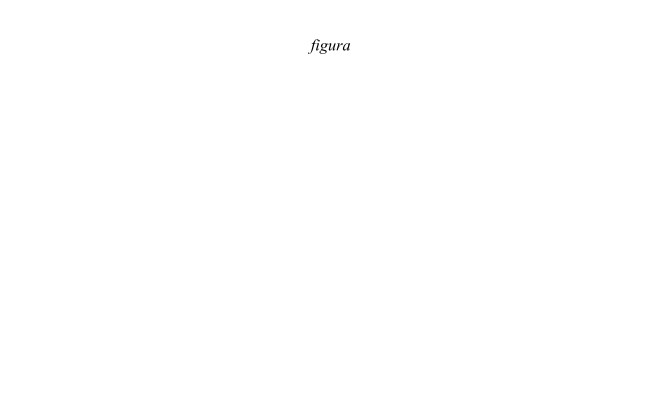
\includegraphics[width=0.98\linewidth]{figs/fig_m.jpg}		
\caption[Utilidade marginal e as curvas de demanda]
{\textbf{---\;Utilidade marginal e as curvas de demanda.}
    Lorem ipsum dolor sit amet consectetur adipiscing elit. Sed ac bibendum orci. Cras erat elit, consequat vel erat ac, tincidunt pulvinar lacus. \;\textbf{a}\;---\;Sed ac bibendum orci. Cras erat elit, consequat vel erat ac, tincidunt pulvinar lacus. Pellentesque vitae consectetur quam. Interdum et malesuada fames ac ante ipsum primis in faucibus.\;\textbf{b}\;---\;Sed ac bibendum orci. Cras erat elit, consequat vel erat ac, tincidunt pulvinar lacus. Pellentesque vitae consectetur quam. Interdum et malesuada fames ac ante ipsum primis in faucibus. \;\textbf{c}\;---\;Sed ac bibendum orci. Cras erat elit, consequat vel erat ac, tincidunt pulvinar lacus. Pellentesque vitae consectetur quam. Interdum et malesuada fames ac ante ipsum primis in faucibus.
}
\label{fig:eco:marginutil} 		
\end{figure}

\par Na \gls{microeon}, o \gls{gutilitarism} encontrou sua expressão máxima na \textbf{\gls{marutilteo}} durante o século XIX, articulada por pensadores como William Stanley Jevons e Carl Menger \cite{Gordon2002a}. Essa \gls{teoria} busca explicar os preços em mercados, entendidos como o resultado de milhares de decisões independentes e descentralizadas entre consumidores e produtores. Ou seja, em um \gls{system} de livre-mercado, a informação sobre a escassez de um recurso é transmitida aos consumidores por meio de seu \textbf{\gls{gprice}}. A \gls{marutilteo} parte da \gls{hipotese} de que o \gls{gprice} consiste no valor de mercado, ou \textbf{\gls{exchaval}}, de um bem ou serviço. Esse valor corresponde à \gls{gutility} adicional que um indivíduo obtém ao consumir uma unidade extra de um bem, a qual diminui conforme o consumo aumenta — o denominado \textbf{\gls{prindecmarut}}. Em termos práticos, isso significa que o consumidor tende a se \textit{saciar} à medida que consome mais de um determinado bem ou serviço. 

\par A \gls{teoria} explica com relativo sucesso o chamado \textbf{\gls{waterdiamonds}}, a bizarra diferença de valor entre diamantes (pouco útil) e água (muito útil).  Nesse caso, o \textbf{\gls{useval}} de um recurso essencial para a sobrevivência como a água pode ser extremamente alto, enquanto seu \gls{exchaval} é relativamente baixo, especialmente onde a água é abundante. Por outro lado, bens como diamantes ou joias têm um \gls{useval} baixo, mas possuem um \gls{exchaval} elevado devido à sua escassez e à alta demanda por aqueles que as consideram itens de status social (mas o \gls{exchaval} é baixo em sociedades que preferem um cocar de penas, por exemplo). Em uma situação de escassez extrema de água, por outro lado, o \gls{exchaval} da água facilmente superar o valor dos diamantes, pois torna-se uma questão de vida ou morte. Esse contraste ilustra como o \gls{useval} e o \gls{exchaval} podem divergir significativamente, e como a \gls{gutility} marginal ajuda a explicar o \gls{gprice} de mercado, independentemente da funcionalidade do bem ou serviço.\footnote{A Teoria do Valor-Trabalho de Karl Marx contrasta com a \gls{marutilteo} ao afirmar que o \textbf{\gls{workval}} de um bem é determinado pelo trabalho socialmente necessário para produzi-lo, e não pela \gls{gutility} que o bem proporciona ao consumidor. Segundo Marx, o valor de um bem é proporcional à quantidade de trabalho incorporado em sua produção, o que inclui tanto o trabalho direto quanto o trabalho necessário para produzir os meios de produção. Esse conceito fundamenta a análise de Marx sobre a exploração do trabalho para se acumular capital, onde os bens são trocados com base no valor do trabalho, mas os trabalhadores recebem apenas uma fração desse valor, criando a mais-valia, ou lucro, para os proprietários dos meios de produção. Ainda que o \gls{workval} de um bem ou serviço possa existir, o problema da tese marxiana é que, na prática, os bens produzidos pelos trabalhadores são vendidos em mercados, pelo \gls{exchaval} auferido pelos consumidores.} Com base nessa lógica, a \gls{teoria} fornece um \gls{model} para explicar (e prever) a formação dos preços nos mercados, e seu conceito de \textbf{\gls{pareteff}} sugere que, sob certas condições, os mercados atingem um equilíbrio, alocando recursos escassos de forma otimizada a satisfazer a todos, sem que seja possível melhorar a situação de alguém sem prejudicar outro.

\par O poder explicativo da \gls{marutilteo} parece corroborar o conceito de \gls{gutility}, já que consumidores e produtores em mercados reais supostamente ajustam suas decisões de acordo com os benefícios marginais -- mesmo sem nunca terem ouvido falar de Jeremy Bentham ou de \gls{gutility} marginal decrescente. Junto com outras teorias auxiliares, a \gls{marutilteo} compõe a base da \gls{microeon} Clássica, que busca explicar cientificamente o funcionamento geral de mercados específicos. Esse conjunto de teorias assume que os agentes na economia são plenamente racionais, capazes de maximizar a sua \gls{gutility} individual, e que os mercados funcionam de maneira eficiente para maximizar a \gls{gutility} total, alcançando um equilíbrio de forma automática, sem intervenções externas. No entanto, para que a suposta eficiência na alocação de recursos seja alcançada, é necessário que não existam \textbf{\gls{marketdist}}, e que condições ideais estejam presentes, como a existência de muitos produtores, disponibilidade total de informações e a ausência de especulação e propaganda — fatores que raramente se verificam na realidade. Além das \gls{marketdist}, o comportamento irracional dos seres humanos, como demonstrado por Daniel Kahneman \cite{kahneman2011}, desafia a ideia de mercados completamente eficientes. Consumidores e produtores, influenciados por vieses cognitivos, como a aversão à perda e o viés de ancoragem, muitas vezes tomam decisões não inteiramente racionais, gerando ineficiências e distorções nos preços. 

\par A \gls{microeon} Evolutiva tenta superar essas limitações ao adotar uma abordagem mais dinâmica, incluindo principalmente simulações com \gls{abm-models} \cite{Bourgine2006a}. Nesse caso, os agentes possuem racionalidade limitada e informações locais, e suas interações ocorrem ao longo do tempo, em processos definidos explicitamente. Além disso, várias instituições, além do mercado, influenciam e sustentam a alocação dos recursos. Assim, a microeconomia evolutiva oferece uma explicação teórica mais robusta para fenômenos que a microeconomia clássica tem dificuldade em justificar. Os \gls{abm-models} da abordagem evolutiva, naturalmente caóticos e computacionalmente irredutíveis, deixam mais claro que, embora ambicionem realizar previsões, as teorias micro-econômicas geralmente se limitam a modelagens exploratórias. Os modelos, assim, trazem uma ampla \gls{explan_cap}, mas pouca \gls{pred_cap}, fazendo a adequação empírica ocorrer em casos muito específicos, geralmente favorecendo algumas das \gls{aux-hyp}, mas não o \gls{model} em sua completude.

\subsection{Paradigmas macroeconômicos} \label{subsec:macroeco}

\par Como mencionado anteriormente, a \gls{macroeon} se diferencia da \gls{microeon} por buscar explicar a economia como um todo, indo além de mercados específicos e abrangendo até a economia nacional e global \cite{samuelson2009}. As doutrinas clássica e neoclássica da \gls{macroeon}, no entanto, tendem a ser uma generalização da \gls{microeon}, expandindo a visão para todos os mercados, produtores e consumidores em uma região de interesse, como um país. O \gls{model} macroeconômico clássico consiste no \textbf{\gls{circflowexval}} entre produtores e consumidores. Na prática, isso corresponde ao fluxo de \gls{exchaval} entre empresas e domicílios, que pode ser medido anualmente pelo faturamento total das empresas e pela renda dos domicílios. Como se trata de um fluxo circular, o valor total de um deve ser equivalente ao do outro. 

\par A escola Neoclássica revisa o \gls{model} clássico ao inserir no \gls{circflowexval} as injeções e vazamentos causados pelas finanças privadas (investimentos e reservas individuais), finanças públicas (arrecadação de impostos) e finanças internacionais (importações e exportações). A maximização da \gls{gutility} total, tido como o \gls{ultimategoal}, pode ser entendida como a maximização desse fluxo de \gls{exchaval} no \gls{system} circular. Portanto, a escola Neoclássica se foca unicamente no fluxo de \gls{exchaval} nos mercados e nas estratégias para aumentá-lo, o que é chamado de \textbf{\gls{ecogrowth}}. As diferenças entre essas estratégias variam, geralmente envolvendo mais ou menos regulação ou intervenção estatal nos mercados de forma a reduzir o desemprego e estabilizar preços. Políticas fiscais e monetárias, por sua vez, objetivam controlar de alguma forma os vazamentos dos impostos e reservas individuais. O sucesso de uma estratégia, porém, é testado pelo aumento no faturamento das empresas ou na renda dos domicílios, sendo esse crescimento interpretado como um sinal de progresso em direção ao \gls{ultimategoal} de maximizar a \gls{gutility} total.

\par A \gls{ecoeco}, articulada principalmente por Herman Daly, propõe um novo \gls{paradigma} que rejeita a escola Neoclássica \cite{daly2011}. Essa visão propõe a \gls{teoria} macroeconômica seja incorporada à \textbf{\gls{ecology}}, uma ciência baseada em princípios físicos, reconhecendo que o \gls{sys-target} a ser modelado é, essencialmente, um \gls{system} material \cite{Daly1968a}. Ao que consta, a perspectiva material sobre a \gls{gseconomics} estava presente nas suas origens Modernas, mas foi lentamente sendo substituída pelo puro interesse no \gls{exchaval}, que é imaterial \cite{Christensen1987}. Um bom exemplo é o de Thomas Malthus (1766-1834), que identificou potenciais limites para o crescimento da população humana em função da produção de alimentos, que cresceria a um ritmo relativamente mais lento. Em essência, Malthus via claramente os seres humanos como seres materiais, que precisam de nutrientes e energia para sobreviver, assim como qualquer outra espécie no planeta. Por exemplo, se um ser humano precisa consumir diariamente 3 litros de água e 0,4 kg de alimentos (aproximadamente 2000 calorias, divididas entre gorduras, carboidratos e proteínas), então se deduz que a população global atual de 8 bilhões de pessoas demanda diariamente 24 milhões de metros cúbicos de água e 50 mil toneladas de alimentos. Sem um fluxo material dessa magnitude, a população global não duraria muito tempo. Oito bilhões parece bastante gente, mas será que seria possível dobrar esse tamanho? Ou triplicar?

\par Uma vez que as previsões de fome generalizada e colapso populacional de Malthus não se concretizaram em sua época, economistas clássicos e neoclássicos tendem a desconsiderar sua \gls{teoria}, confundindo suas conclusões circunstanciais com os fundamentos materiais de sua abordagem. No debate acirrado que surgiu com a proposta da \gls{ecoeco}, economistas neoclássicos acusam os proponentes do novo \gls{paradigma} de serem \say{neomalthusianos}, o que soa um tanto de forma pejorativa \cite{Forrester1974}. A visão ecológica, por sua vez, acusa a escola Neoclássica em se focar excessivamente nos fluxos de \gls{exchaval} de \textbf{\gls{marktegoods}}, bens e serviços muito específicos que podem ser comprados ou vendidos \cite{Daly1997a, Daly1997b}. Esse foco no fluxo de valor é tão hegemônico que a escola Neoclássica sequer considera a materialidade das \gls{marktegoods}: elas são apenas \textit{veículos} que transportam \gls{gutility} marginal, definida pelo seu \gls{gprice}. Assim, a escola Neoclássica instancia uma ontologia imaterial e abstrata de \gls{exchaval}. Essa representação pode ser um \gls{model} interessante para entender e explicar os fluxos de valores em mercados, mas nem de perto consiste em uma representação de uma realidade material.

\subsection{A ontologia do Fisicalismo} \label{subsec:physicalism}

\begin{figure}[t!] 
\centering				
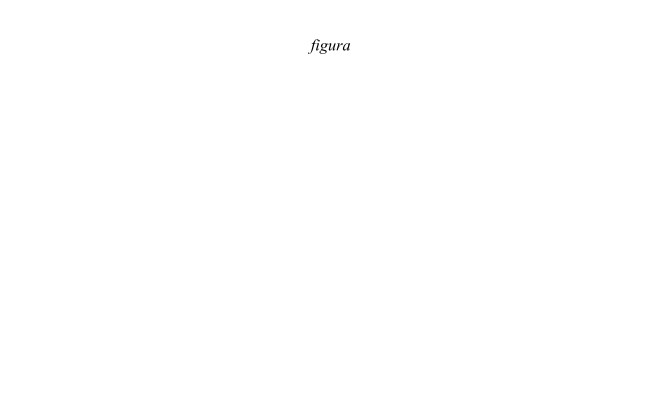
\includegraphics[width=0.98\linewidth]{figs/fig_m.jpg}		
\caption[A ontologia Fisicalista]
{\textbf{---\;A ontologia Fisicalista.}
    Lorem ipsum dolor sit amet consectetur adipiscing elit. Sed ac bibendum orci. Cras erat elit, consequat vel erat ac, tincidunt pulvinar lacus. \;\textbf{a}\;---\;Sed ac bibendum orci. Cras erat elit, consequat vel erat ac, tincidunt pulvinar lacus. Pellentesque vitae consectetur quam. Interdum et malesuada fames ac ante ipsum primis in faucibus.\;\textbf{b}\;---\;Sed ac bibendum orci. Cras erat elit, consequat vel erat ac, tincidunt pulvinar lacus. Pellentesque vitae consectetur quam. Interdum et malesuada fames ac ante ipsum primis in faucibus. \;\textbf{c}\;---\;Sed ac bibendum orci. Cras erat elit, consequat vel erat ac, tincidunt pulvinar lacus. Pellentesque vitae consectetur quam. Interdum et malesuada fames ac ante ipsum primis in faucibus.
}
\label{fig:eco:physicalism} 		
\end{figure}

\par Em termos ontológicos, a \gls{ecoeco} sustenta uma realidade fisicalista. O \textbf{\gls{gphysicalism}}\footnote{Também denominado de Materialismo.} é uma corrente de pensamento realista e naturalista que postula que a realidade objetiva existe, rege-se pelas leis da Física e é composta em última instância de matéria e energia \cite{sep-physicalism}. Sendo a Física uma \gls{teoria} científica, o \gls{gphysicalism} consiste na principal visão de mundo diretamente implicada pelo Realismo Científico. Nessa perspectiva, até mesmo o conceito de \gls{gutility} consiste em algo material, pois coisas como \say{bem-estar} ou \say{satisfação} na verdade são sinapses em cérebros, um órgão do corpo humano. 

\par O \gls{gphysicalism}, apesar de atrativo devido à sua forte adequação empírica, enfrenta alguns problemas estruturais críticos. Um dos principais é o problema mente-corpo, ou o \textbf{\gls{consproblem}} — a aparente impossibilidade de se explicar as experiências subjetivas a partir de processos físicos, como as sinapses \cite{sep-consciousness}. Outro problema grave é o \textbf{\gls{willproblem}}, que surge ao se aceitar as últimas consequências do \gls{gphysicalism}, que é o Determinismo \cite{sep-skepticism}. Em uma realidade determinista, decisões seriam meras sensações, sem agência real, tornando a ideia de escolhas na alocação de recursos, central na \gls{gseconomics}, desprovida de qualquer sentido\footnote{O \gls{gphysicalism} radical conduz ao Niilismo, uma \gls{teoria} ética que nega a existência de valores morais ou objetivos supremos para orientar decisões}. Mas ambos os problemas são sintomas do Realismo Científico, que propõe que a Ciência busca descrever a verdade sobre a realidade. Os Instrumentalistas, como Bas van Fraassen e Nancy Cartwright, contestam essa visão, argumentando que as teorias científicas objetivam apenas descrições empiricamente adequadas, sem necessariamente refletir a verdade última sobre o mundo \cite{bas1980, nancy1983}. Nesse sentido, escolher uma ontologia fisicalista para a \gls{macroeon} oferece uma base empiricamente mais robusta do que a escola Neoclássica, cuja explicação se limita ao fluxo de \gls{exchaval} nos mercados. Verdadeira ou não, uma base física oferece maior \gls{explan_cap} e preditiva do que o \gls{model} de fluxo circular neoclássico.

\par Um dos pioneiros a aceitar e difundir o \gls{gphysicalism} na \gls{gseconomics}, preparando o terreno para o \gls{paradigma} ecológico, foi Nicholas Georgescu-Roegen (1906-1994), especialmente com sua obra seminal \textit{A Lei da Entropia e o Processo Econômico}\footnote{Tradução livre de \textit{The Entropy Law and the Economic Process}} (1971). Nessa obra, Georgescu-Roegen destaca as implicações da primeira e da segunda leis da termodinâmica em uma economia baseada em recursos materiais. A \textbf{\gls{firstlaw}}, conhecida como o \textbf{princípio da conservação}, afirma que matéria e energia não podem ser criadas nem destruídas, apenas transformadas de uma forma para outra. Já a \textbf{\gls{secondlaw}} estabelece que a \textbf{entropia} de um \gls{system} isolado tende a aumentar, indicando que os processos naturais seguem uma trajetória de desordem crescente. Isso significa que a \textbf{energia livre}, capaz de realizar trabalho, tende a se degradar em formas cada vez menos capazes de realizar trabalho. Da mesma maneira, as estruturas materiais tendem a se desintegrar espontaneamente de um estado ordenado (heterogêneo e menos provável) para um estado desordenado (homogêneo e mais provável). A segunda lei implica também que nenhum processo de transferência de energia ou conversão material é 100\% eficiente, pois sempre ocorrerão perdas na forma de calor e resíduos. Portanto, essas leis estabelecem que a manutenção de ordem no Universo só é possível localmente e às custas de fontes externas de energia livre. Mesmo assim, a criação de ordem por meio de trabalho resulta inevitavelmente na geração de resíduos materiais e energéticos sem \gls{gutility}.

\par Outro pioneiro na visão fisicalista foi Jay Forrester, o inventor da \gls{sys-dyn}, tema introduzido no Capítulo \ref{chap:systems}. Jay Forrester e a sua equipe de engenheiros e cientistas no \texttt{MIT} demonstraram a partir das publicações \textit{World Dynamics} e \textit{Limites do crescimento} como que modelos de compartimentos podem ser empregados para se obter previsões sobre o estado da economia global ao longo do tempo \cite{Forrester1973a, meadows1974}. As simulações do \gls{model} \texttt{World3} introduziram uma abordagem fisicalista, demonstrando a materialidade do \gls{system} econômico ao integrar os níveis e fluxos materiais dos \gls{system} global, tais como a população, capital industrial, terras agricultáveis e a poluição resultante. Os resultados, ainda que variados para diferentes cenários, evidenciam os limites físicos impostos pela \gls{biosf} sobre a \gls{antroposf}, como o esgotamento de fontes energéticas não-renováveis, a degradação de terras agrícolas e a capacidade finita de absorção de poluentes dos ecossistemas. Nos diversos cenários explorados, o crescimento da população humana e de capital industrial enfrentam inevitavelmente um ponto de ruptura, onde o aumento dos custos de extração de recursos, a perda de produtividade agrícola e os impactos da poluição aplicam retroações negativas cada vez maiores, resultando cedo ou tarde em um declínio no crescimento de capital industrial. Assim, as explorações do \texttt{World3} ilustraram a interdependência entre o \gls{system} econômico e os limites físicos da \gls{biosf}.

\subsection{O modelo ecológico} \label{subsec:ecomodel}

\begin{figure}[t!] 
\centering				
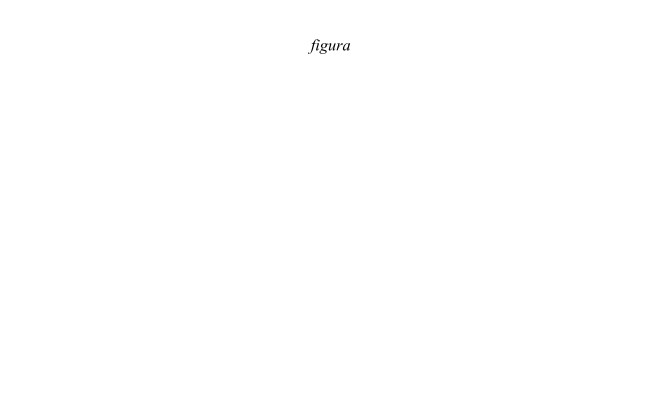
\includegraphics[width=0.98\linewidth]{figs/fig_m.jpg}		
\caption[A \gls{macroeon} Ecológica]
{\textbf{---\;A \gls{macroeon} Ecológica.}
    Lorem ipsum dolor sit amet consectetur adipiscing elit. Sed ac bibendum orci. Cras erat elit, consequat vel erat ac, tincidunt pulvinar lacus. \;\textbf{a}\;---\;Sed ac bibendum orci. Cras erat elit, consequat vel erat ac, tincidunt pulvinar lacus. Pellentesque vitae consectetur quam. Interdum et malesuada fames ac ante ipsum primis in faucibus.\;\textbf{b}\;---\;Sed ac bibendum orci. Cras erat elit, consequat vel erat ac, tincidunt pulvinar lacus. Pellentesque vitae consectetur quam. Interdum et malesuada fames ac ante ipsum primis in faucibus. \;\textbf{c}\;---\;Sed ac bibendum orci. Cras erat elit, consequat vel erat ac, tincidunt pulvinar lacus. Pellentesque vitae consectetur quam. Interdum et malesuada fames ac ante ipsum primis in faucibus.
}
\label{fig:eco:ecomodel} 		
\end{figure}

\par A partir das leis termodinâmicas e da visão sistêmica, a \gls{ecoeco} representa a macroeconomia por um \gls{model} ecológico. Nesse \gls{model}, a \textbf{\gls{antroposf}} – o ambiente material habitado pelos seres humanos – está inserida na \textbf{\gls{biosf}}, que abrange o \gls{system} material da superfície da Terra, desde a atmosfera até os primeiros quilômetros subterrâneos da litosfera. Energeticamente, a \gls{biosf} não é um \gls{system} isolado, mas aberto, recebendo um fluxo contínuo de energia livre da radiação do sol e do núcleo interno do planeta. Essa energia de alta qualidade, após realizar trabalho, é emitida para o espaço em formas menos úteis de calor. Materialmente, a \gls{biosf} também está conectada a fluxos de entrada e saída promovidos pelos processos de subducção, soterramento, soerguimento e vulcanismo, que resultam dos movimentos de convecção do manto, além das perdas de gases leves para o espaço. Embora processos como o vulcanismo representem exceções mais súbitas, a maioria das trocas materiais na \gls{biosf} ocorre de maneira extremamente lenta, em escalas geológicas. Dessa forma, a \gls{biosf} pode ser considerada, na prática, um \gls{system} energeticamente aberto, mas materialmente fechado.

\par A abertura energética de um \gls{system} é fundamental para a criação de ordem no seu interior. A fotossíntese, por exemplo, é um dos principais processos de geração de ordem na \gls{biosf}, ao empregar a energia livre da radiação solar para produzir materiais de baixa entropia, como açúcares, a partir de compostos de alta entropia, como o dióxido de carbono. Processos de soterramento desses materiais de baixa entropia ao longo de milhões de anos produziram as reservas de combustíveis fósseis amplamente utilizadas hoje pela \gls{antroposf}. Além da fotossíntese, o motor do ciclo do carbono, diversos outros \textbf{ciclos bio-geoquímicos} ocorrem na \gls{biosf}, todos impulsionados por fontes externas de energia. O \gls{hydro_cicle}, por exemplo, é movido pela energia solar, que evapora a água e a eleva, conferindo-lhe potencial gravitacional, que pode realizar trabalho em moinhos ou turbinas. Esses ciclos mantêm a dinâmica e a ordem da \gls{biosf}, demonstrando a interdependência entre o aporte de energia externa e a organização interna do \gls{system}.

\par Os fundamentos físicos da \gls{ecoeco} resulta em uma interpretação completamente diferente de \gls{ecogrowth}. A \gls{firstlaw}, vista sob a lente do \gls{model} ecológico, implica que não existe crescimento material real na \gls{biosf}, uma vez que a matéria se conserva. A \gls{antroposf}, sendo um habitat humano dentro da \gls{biosf}, pode expandir a sua complexidade estrutural ao processar os materiais da \gls{biosf}, mas sempre às custas da geração de calor e outros resíduos. A \gls{secondlaw}, por sua vez, implica que a mera \textit{sustentação} da atroposfera exige um fluxo de energia livre e de materiais de reposição, pois é necessário trabalhar continuamente contra a degradação espontânea do \gls{system} material. Esse fluxo inevitável de matéria que é processada pela \gls{antroposf} e gera resíduos inúteis dispersos na \gls{biosf} é chamado na \gls{ecoeco} de \textbf{\gls{gthoughput}}\footnote{Tradução livre de \textit{throughput}.}. Nesse sentido, o \gls{ecogrowth} teorizado pela \gls{gseconomics} Neoclássica é, sobretudo, uma ilusão, um fenômeno imaginário instanciado pela realidade intersubjetiva do \gls{exchaval}. Mas como bens e serviços em mercados são entidades materiais, aumentar o seu consumo implica, obrigatoriamente, em aumentar o \gls{gthoughput}. A diferença entre os paradigmas econômicos, aqui, torna-se muito clara: enquanto um instancia um fluxo circular e imaterial (\gls{gutility} marginal e valor de troca), o outro vê um fluxo linear e material (processamento de energia livre).

\section{Capital natural} \label{chap:ecoeco:natcap}

\subsection{A escala ótima da antroposfera} \label{subsec:escaleopt}

\begin{figure}[t!] 
\centering				
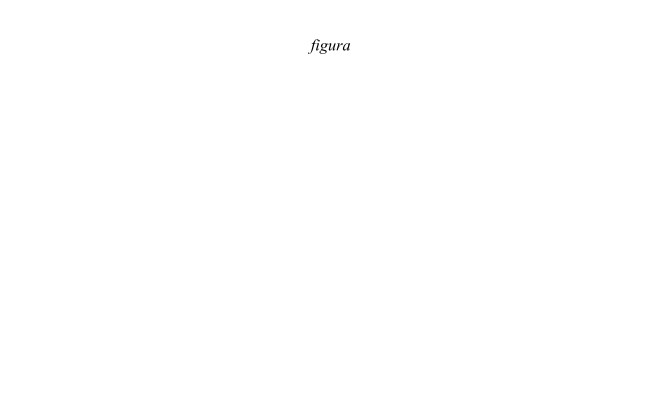
\includegraphics[width=0.98\linewidth]{figs/fig_m.jpg}		
\caption[A escala ótima da Antroposfera]
{\textbf{---\;A escala ótima da Antroposfera.}
    Lorem ipsum dolor sit amet consectetur adipiscing elit. Sed ac bibendum orci. Cras erat elit, consequat vel erat ac, tincidunt pulvinar lacus. \;\textbf{a}\;---\;Sed ac bibendum orci. Cras erat elit, consequat vel erat ac, tincidunt pulvinar lacus. Pellentesque vitae consectetur quam. Interdum et malesuada fames ac ante ipsum primis in faucibus.\;\textbf{b}\;---\;Sed ac bibendum orci. Cras erat elit, consequat vel erat ac, tincidunt pulvinar lacus. Pellentesque vitae consectetur quam. Interdum et malesuada fames ac ante ipsum primis in faucibus. \;\textbf{c}\;---\;Sed ac bibendum orci. Cras erat elit, consequat vel erat ac, tincidunt pulvinar lacus. Pellentesque vitae consectetur quam. Interdum et malesuada fames ac ante ipsum primis in faucibus.
}
\label{fig:eco:escaleopt} 		
\end{figure}

\par Embora a \gls{ecoeco} rejeite as ideias neoclássicas no campo da \gls{macroeon}, ela compartilha vários conceitos fundamentais da \gls{microeon}, como a \gls{marutilteo} e o \gls{ultimategoal} de maximização do \gls{welbeing}. Nesse sentido, Herman Daly propõe que, sendo a \gls{antroposf} um sub\gls{system} material da \gls{biosf}, existe uma \textbf{escala ótima} para a \gls{antroposf}, ponto em que o \gls{welbeing} atinge seu máximo \cite{Daly2015a}. Após o chamado \textbf{\gls{ecolimit}}, o crescimento da \gls{antroposf} se torna anti-econômico, gerando prejuízos crescentes. O conceito de \textbf{\gls{sustdev}} está diretamente ligado a essa ideia, indicando que o crescimento material da economia deve ser balanceado dentro dos limites da \gls{biosf}. Assim, as escolhas econômicas precisam considerar esse equilíbrio, implementando mecanismos e políticas que evitem que a \gls{antroposf} ultrapasse seu ponto ótimo. O programa de pesquisa do \gls{paradigma}, portanto, objetiva investigar quão próximo estamos desse limite. Em um mundo vazio, há espaço para expandir. Já em um mundo lotado, esse limite pode ter sido ultrapassado, exigindo um planejamento que priorize o \textbf{decrescimento} da \gls{antroposf}.

\par O entendimento da escala ótima só é possível ao se generalizar o conceito de \textit{capital} para além da sua concepção convencional. Na visão ecológica, \textbf{\gls{antcap}} consiste nas estruturas materiais e sociais construídas por seres humanos que produzem um fluxo de bens e serviços, resultando em \gls{welbeing}. A definição é vaga e pode ser confundido com a própria \gls{antroposf}. Uma fábrica de motocicletas, por exemplo, consiste em um típico exemplar de capital industrial que produz bens (motocicletas). Uma motocicleta, contudo, pode ser usada para fornecer um serviço de entrega, o que a torna um bem por um lado e um capital por outro. A capacidade de pilotar uma motocicleta faz dos trabalhadores de uma empresa de entregas o seu capital humano. O termo \say{capitalismo}, nesse sentido, consiste na doutrina de acumulação de \gls{antcap}, ou de expansão da \gls{antroposf}. Note-se que, na ótica neoclássica, o capitalismo explicitamente determina o crescimento do capital, mas apenas indiretamente assume que isso irá aumentar o bem-humano, pelo aumento do fluxo de \gls{exchaval}. Como vimos acima, essa doutrina resulta na expansão da \gls{antroposf} sobre a \gls{biosf}, aumentando o \gls{gthoughput}. 

\par Mas além do \gls{antcap}, a visão ecológica também instancia o conceito de \textbf{\gls{natcap}}. A ideia foi articulada inicialmente por Robert Costanza e Herman Daly, em \gls{analogy} ao capital construído \cite{Costanza1992a}. Assim, o \gls{natcap} se define pelas estruturas materiais da própria \gls{biosf} que produzem um fluxo \textit{direto} de bens e serviços, resultando em \gls{welbeing}. Além de bens diretamente utilizáveis, como madeira ou um cardume de peixes, também são considerados serviços, como a polinização, que sustenta a produção de alimentos, a formação de solos férteis, indispensável para a agricultura, e os ciclos biogeoquímicos, como o sequestro de carbono, que regula o clima global. Esses serviços resultam de \textbf{funções ambientais} fundamentais para a vida na Terra, ainda que negligenciados pela abordagem convencional sobre \gls{natrec} \cite{Groot1987a}. Um bom exercício para ilustrar sua importância é imaginar o que seria necessário construir para reproduzir as condições naturais em uma colônia humana em Marte. Sem o suporte do \gls{natcap}, todos os processos essenciais à vida teriam que ser artificialmente replicados, evidenciando a interdependência crítica entre a \gls{antroposf} e a \gls{biosf}.

\par O cerne do conceito de escala ótima, portanto, é reconhecer que a construção de \gls{antcap} exige a desmontagem da infraestrutura existente de \gls{natcap}. Isso resulta obrigatoriamente em um sacrifício de bem-estar provido diretamente pelos recursos e \gls{natserv}. No jargão econômico, existe um \textbf{\gls{opcost}} na expansão da \gls{antroposf}, que é o sacrifício dos recursos e \gls{natserv} providenciados pelo \gls{natcap}. A \gls{marutilteo}, ajuda a ilustrar esse dilema pelo diagrama de \gls{gutility} (Figura [ref]): o \gls{ecolimit} do crescimento do \gls{antcap} ocorre quando a sua \gls{gutility} marginal se iguala à sua \textbf{\gls{desutilmar}}. A \gls{desutilmar} consiste na perda incremental de \gls{gutility} do lado do \gls{natcap}, e consiste exatamente no \gls{opcost}. Essa perda incremental de \gls{gutility} é pequena em um mundo vazio: uma pequena clareira aberta em uma imensa floresta é praticamente imperceptível em termos de prejuízos, mesmo na \gls{loc-scale} do ecos\gls{system}. Mas à medida o mundo torna-se lotado, as perdas de \gls{gutility} crescem de forma não linear. Em certos casos, é possível que um \textbf{\gls{colaplimit}} possa ser superado, quanto processos de degradação praticamente irreversíveis passam a ser desencadeados. O diagrama representa a totalidade da \gls{biosf}, mas também pode ser interpretado outras escalas, como em países, bacias, etc, e em relação a processos naturais específicos. Em uma bacia hidrográfica, por exemplo, o \gls{ecolimit} seria uma ocupação do solo e uso da água equilibrada, que preserva diversos outros bens e \gls{natserv}. Um exemplo mais intuitivo é o \gls{system} do clima global: o \gls{ecolimit} seria um nível de poluição por gases de efeito estufa que se compensaria em termos de bem-estar, enquanto que o \gls{colaplimit} representa um nível de poluição em que os processos de mudança climática tornam-se descontrolados, ativando retroações positivas. 

\par O \gls{ecolimit} e o \gls{colaplimit} são em geral inferiores ao \textbf{\gls{futilelimit}}, o nível em que a \gls{gutility} marginal do \gls{antcap} é nula ou mesmo negativa (a situação quando mais recursos trazem diretamente \textit{menos} bem-estar). Isso traz implicações políticas importantes, que confrontam o \textit{status quo} social. A escola econômica Neoclássica tende a ser bem-vista pelas elites sociais, pois ela sugere que basta aumentar o consumo dos recursos para se aumentar o bem-estar coletivo, independentemente das desigualdades relativas entre os consumidores. Com chamada \textbf{promessa da fatia maior} , basta fazer o \say{bolo} crescer para todos que os mais pobres terão amanhã uma fatia maior que hoje – ainda que o fatiamento continue sendo injusto. Mas ao se admitir que existe uma escala ótima para a \gls{antroposf}, vemos que os recursos devem ser consumidos no \gls{ecolimit} para se maximizar o \gls{welbeing}, muito abaixo do \gls{futilelimit}. A única possibilidade viável de alguém consumir recursos acima do \gls{ecolimit} é garantir que outros consumam muito abaixo, um compensando a perda de \gls{natcap} do outro. Mas como esse arranjo desigual não maximiza o bem-estar coletivo, a \gls{ecoeco} postula que, em um mundo material finito, a desigualdade é imoral.  

\subsection{Compreendendo os recursos naturais} \label{subsec:natrec}

\begin{figure}[t!] 
\centering				
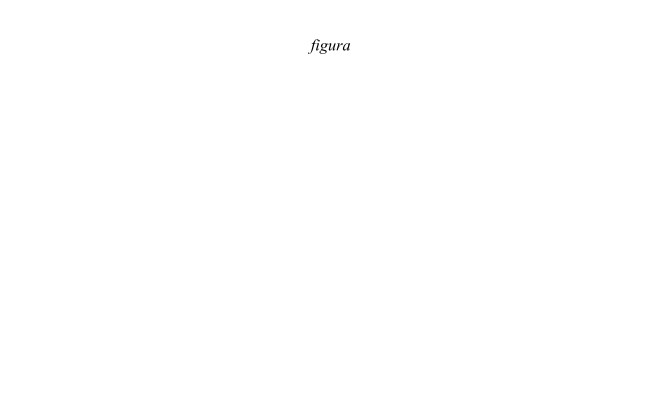
\includegraphics[width=0.98\linewidth]{figs/fig_m.jpg}		
\caption[Classificação dos recursos naturais]
{\textbf{---\;Classificação dos \gls{natrec}.}
    Lorem ipsum dolor sit amet consectetur adipiscing elit. Sed ac bibendum orci. Cras erat elit, consequat vel erat ac, tincidunt pulvinar lacus. \;\textbf{a}\;---\;Sed ac bibendum orci. Cras erat elit, consequat vel erat ac, tincidunt pulvinar lacus. Pellentesque vitae consectetur quam. Interdum et malesuada fames ac ante ipsum primis in faucibus.\;\textbf{b}\;---\;Sed ac bibendum orci. Cras erat elit, consequat vel erat ac, tincidunt pulvinar lacus. Pellentesque vitae consectetur quam. Interdum et malesuada fames ac ante ipsum primis in faucibus. \;\textbf{c}\;---\;Sed ac bibendum orci. Cras erat elit, consequat vel erat ac, tincidunt pulvinar lacus. Pellentesque vitae consectetur quam. Interdum et malesuada fames ac ante ipsum primis in faucibus.
}
\label{fig:eco:natrec} 		
\end{figure}

\par A classificação dos \textbf{\gls{natrec}} pela \gls{ecoeco} contrasta fortemente com a abordagem da escola Neoclássica. Como a \gls{macroeon} Neoclássica tende a ser uma visão estendida da \gls{microeon}, esse \gls{paradigma} trata os recursos de forma homogênea, reduzindo eles a meros insumos, ou \textbf{fatores de produção}, que contribuem para a maximização de bens e serviços pelo \gls{antcap}. Em geral, os fatores são categorizados em \say{terra} (matérias-primas) e \say{trabalho} (mão de obra), além do próprio capital (máquinas e equipamentos). Na visão Neoclássica, prevalece a ideia de  \textbf{capacidade de substituição}, ou seja, a possibilidade de trocar um insumo por outro quando este estiver escasso, o que gera uma relativa insensibilidade ao esgotamento dos recursos utilizados. Por não reconhecer a existência de \gls{natcap}, o esgotamento de matérias-primas não é considerado um problema de base, desde que possam ser substituídas com o advento de inovações tecnológicas. 

\par Não obstante, Herman Daly articula uma distinção crítica entre \textbf{\gls{recstflow}}, que podem ser consumidos em qualquer ritmo, e os \textbf{\gls{fundserv}}, cuja produtividade é limitada no tempo e que não podem ser facilmente substituídos \cite{daly2011}. O \gls{natcap} pode ser de um tipo ou de outro. Mas também pode ser ambos, como no caso das florestas. As florestas são um estoque-fluxo de madeira, uma matéria-prima. Mas também são um fundo-serviço de diversos \textbf{\gls{natserv}}. Com isso, o \gls{scale_problem} ótima se faz evidente: o \gls{econbenefit} de desmontar uma floresta vem junto com o \gls{opcost} dos \gls{natserv} sacrificados. Mas como as florestas são um \gls{system} que se regenera com energia do sol, é possível encontrar um fluxo sustentável de obtenção de madeira sem abrir completamente mão dos \gls{natserv}. Essa classificação ressalta a necessidade de estratégias que levem em consideração os limites e a insubstituibilidade de certos recursos, oferecendo uma estrutura mais adequada para se desenhar políticas de \gls{sustdev}.

\par Os \gls{recstflow} são aqueles que são materialmente transformados durante o processo produtivo, ou seja, tornam-se parte do produto final. No contexto do \gls{natcap}, esses recursos são classificados como \textbf{\gls{recrenew}} e \textbf{\gls{recnotrenew}}. Um exemplo claro é o petróleo, que é refinado em combustível, ou as árvores, que são convertidas em tábuas e papel. Quando disponíveis, esses recursos podem ser consumidos a praticamente qualquer ritmo. Por exemplo, grandes quantidades de petróleo podem ser extraídas rapidamente, desde que existam poços suficientes e refinarias em operação. De forma semelhante, uma floresta pode ser desmatada em poucos dias, se houver máquinas e trabalhadores suficientes. Esses recursos também podem ser estocados para uso futuro; matérias-primas como grãos, combustíveis e minerais podem ser armazenados em depósitos, permitindo um gerenciamento flexível ao longo do tempo. Similarmente, talhões de florestas podem ser preservados para corte em ocasiões futuras. 

\par Quando consumidos a uma velocidade maior que a \textbf{\gls{carycap}}, os \gls{recstflow} se esgotam subitamente. Como o petróleo leva milhões de anos para se formar naturalmente, ele é considerado um recurso não renovável, assim como a maioria dos \textbf{\gls{recmineral}}. Já as florestas, quando manejadas adequadamente, podem se regenerar em um período razoavelmente curto de tempo, o que torna a madeira das árvores um recurso renovável, assim como a maioria dos \textbf{\gls{recbio}}. A água, apesar de ser um \textbf{\gls{recabio}}, também é um recurso renovável, pois o \gls{hydro_cicle} atua constantemente, eventualmente regenerando os níveis dos rios e lagos.  Contudo, uma vez utilizados, esses recursos são destruídos e não podem ser recuperados em sua forma original. Em certos casos, os resíduos gerados podem ser reutilizados em outros processos ou reciclados. A identificação de \textbf{\gls{recreus}} e \textbf{\gls{recreci}} consiste em uma estratégia essencial para a sustentabilidade, pois reduz o \gls{gthoughput} na \gls{antroposf}. Ainda assim, é preciso lembrar que esses processos não reduzem a necessidade de importar energia livre para a realização de trabalho.

\par Por outro lado, \gls{fundserv} são aqueles que participam do processo produtivo \textit{sem} se transformarem fisicamente no produto final. Eles fornecem os meios e serviços essenciais para o processo produtivo, mas não se esgotam de imediado. A destruição desses recursos ocorre pelo desgaste ou \textbf{\gls{deprec}} ao longo do tempo, pela ação da \gls{secondlaw}. No caso do \gls{antcap}, infraestruturas como rodovias, sistemas energéticos, redes de comunicação, além de máquinas e mão de obra, são exemplos desses recursos. Eles não se tornam parte do produto final; uma máquina de costura, por exemplo, participa da fabricação de roupas, mas não se incorpora no produto. Em contraste com os \gls{recstflow}, os \gls{fundserv} têm uma capacidade limitada de produção por unidade de tempo. Uma máquina ou um trabalhador pode produzir apenas uma quantidade finita de produtos em um determinado período, independentemente da quantidade de matéria-prima disponível. Além disso, esses serviços não podem ser estocados. Se uma fábrica fica inativa por uma semana, a capacidade produtiva dessa semana é perdida e não pode ser recuperada posteriormente. Com o tempo, esses recursos se desgastam; uma máquina, por exemplo, enferruja e precisa de manutenção, e os trabalhadores necessitam de descanso e capacitação contínua para manter a sua produtividade. Por isso, esses recursos não existem de forma estática, mas também participam no \gls{gthoughput}, consumindo energia livre e materiais de baixa entropia.

\par Ao contrário do \gls{antcap}, que depende de manutenção contínua por intervenções humanas, o \gls{natcap} possui intrínsecos mecanismos de \textbf{\gls{selforg}}. Os ciclos biogeoquímicos, por exemplo, são impulsionados por fontes de energia livres como a radiação solar e o calor do núcleo terrestre, tornando a \gls{biosf} um \gls{system} auto-organizado que sustenta a vida e regula os fluxos de materiais e energia. Como veremos adiante com mais detalhes, os \gls{natserv} são os \gls{fundserv} que obtemos diretamente desse \gls{system} autorregulado. Esses serviços podem ser categorizados em três grandes grupos: os \textbf{\gls{natservprov}}, que abrangem a capacidade da \gls{biosf} de fornecer e regenerar \gls{recstflow}, como alimentos, água e matérias-primas; os \textbf{\gls{natservreg}}, que controlam processos vitais como o ciclo da água, a regulação do clima e a polinização, equilibrando e organizando os fluxos materiais dentro da \gls{biosf}; e os \textbf{\gls{natservcult}}, que se referem ao bem-estar imaterial proporcionado pela interação humana direta com o ambiente natural, seja através de atividades recreativas, científicas, religiosas ou espirituais. Exemplos concretos desses serviços incluem a capacidade de florestas tropicais de sequestrar carbono da atmosfera, regulando o clima global, ou os recifes de corais, que não só fornecem habitats para uma vasta biodiversidade marinha, mas também servem como barreiras naturais contra tempestades costeiras. Da mesma forma, a interação com paisagens naturais, como parques nacionais, promove a saúde mental e o \gls{welbeing}, exemplificando a dimensão cultural desses serviços.

\subsection{O problema do livre acesso} \label{subsec:tragedy}

\begin{figure}[t!] 
\centering				
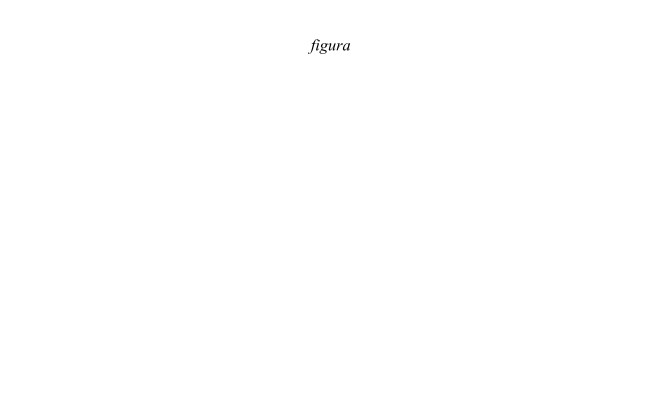
\includegraphics[width=0.98\linewidth]{figs/fig_m.jpg}		
\caption[Soluções para o problema do livre acesso]
{\textbf{---\;Soluções para o \gls{probfreeacc}.}
    Lorem ipsum dolor sit amet consectetur adipiscing elit. Sed ac bibendum orci. Cras erat elit, consequat vel erat ac, tincidunt pulvinar lacus. \;\textbf{a}\;---\;Sed ac bibendum orci. Cras erat elit, consequat vel erat ac, tincidunt pulvinar lacus. Pellentesque vitae consectetur quam. Interdum et malesuada fames ac ante ipsum primis in faucibus.\;\textbf{b}\;---\;Sed ac bibendum orci. Cras erat elit, consequat vel erat ac, tincidunt pulvinar lacus. Pellentesque vitae consectetur quam. Interdum et malesuada fames ac ante ipsum primis in faucibus. \;\textbf{c}\;---\;Sed ac bibendum orci. Cras erat elit, consequat vel erat ac, tincidunt pulvinar lacus. Pellentesque vitae consectetur quam. Interdum et malesuada fames ac ante ipsum primis in faucibus.
}
\label{fig:eco:tragedy} 		
\end{figure}

\par Desenhar políticas de alocação de recursos para manter a \gls{antroposf} no seu \gls{ecolimit} passa invariavelmente por endereçar o \textbf{\gls{probfreeacc}}. Esse problema foi articulado no artigo \textit{A tragédia dos comuns} pelo ecólogo Garret Hardin (1968) \cite{Hardin1968a}. Nesse artigo, Hardin argumenta que os problemas ambientais, como o sobreuso da terra e a poluição da água, são consequência do livre acesso de bens e serviços que são de uso comum, ou \textbf{\gls{reccom}}\footnote{Esse termo refere-se tanto ao \gls{natcap} quanto ao \gls{antcap}.}. Como os indivíduos e empresas agem para maximizar apenas o seu bem-estar individual, o livre acesso acaba criando uma corrida desenfreada para aproveitar o recurso, que acaba sendo congestionado ou esgotado. Configura-se uma tragédia, portanto, pois a ação supostamente racional dos indivíduos termina por ser um movimento irracional do coletivo. Hardin reconhece, com isso, que fazer do recurso público um bem análogo a recursos privados pode ser uma solução interessante, mas que não se aplica em todos os casos:

\begin{adjustwidth}{100pt}{0pt}
\medskip
\small A tragédia dos comuns, entendida como uma cesta de alimentos, é evitada pela \gls{privprop}, ou algo formalmente semelhante. Mas o ar e as águas ao nosso redor não podem ser facilmente cercados, e assim a tragédia dos comuns, entendida como uma fossa séptica, deve ser evitada por outros meios, através de leis coercitivas ou dispositivos de taxação que tornem mais barato para o poluidor tratar seus poluentes do que descartá-los sem tratamento. Não avançamos tanto na solução desse problema quanto no primeiro. De fato, nosso conceito particular de \gls{privprop}, que nos impede de esgotar os recursos da Terra, favorece a poluição. O proprietário de uma fábrica na margem de um rio — cuja propriedade se estende até o meio do rio — muitas vezes tem dificuldade em entender por que não é seu direito natural poluir as águas que passam por sua porta. A lei, sempre desatualizada, exige uma adaptação elaborada para se ajustar a este aspecto recentemente percebido dos bens comuns.\footnote{
Tradução livre de: \textit{The tragedy of the commons as a food basket is averted by private property, or something formally like it. But the air and waters surrounding us cannot readily be fenced, and so the tragedy of the commons as a cesspool must be prevented by different means, through coercive laws or taxing devices that make it cheaper for the polluter to treat their pollutants than to discharge them untreated. We have not progressed as far with the solution to this problem as we have with the first. Indeed, our particular concept of private property, which deters us from exhausting the positive resources of the earth, favors pollution. The owner of a factory on the bank of a stream—whose property extends to the middle of the stream—often has difficulty seeing why it is not their natural right to muddy the waters flowing past their door. The law, always behind the times, requires elaborate stitching and fitting to adapt it to this newly perceived aspect of the commons.}
} -- Garret Hardin (1968, p. 1245) \cite{Barnes1939}.
\medskip
\end{adjustwidth}

\noindent O problema da poluição da água e do ar pode ser resolvido ao impor que os poluidores assumam total responsabilidade por seus resíduos. Um conceito central da \gls{microeon} Neoclássica, nesse sentido, é o de \textbf{\gls{external}}, que pode ser positiva ou negativa. Externalidade refere-se ao impacto das ações de um agente econômico sobre o bem-estar de outros \cite{Mankiw2002a}. No exemplo de Hardin, em que uma fábrica polui o ar e a água, devem ser criados mecanismos regulatórios para evitar a perda de bem-estar coletivo (a \gls{external} negativa), obrigando a fábrica a gerir seus resíduos, mesmo que isso seja mais oneroso. Nesse contexto, a \gls{ecoeco} oferece uma interpretação mais ampla do \gls{probfreeacc} e das externalidades em comparação com a \gls{microeon} Neoclássica. O conceito de \gls{external} negativa, segundo essa visão, está relacionado ao \gls{opcost} da expansão da \gls{antroposf} sobre a \gls{biosf}. A transformação de um rio em um canal de efluentes gera uma série de externalidades negativas precisamente pela perda de \gls{natcap} -- os recursos e serviços diretamente fornecidos pelo rio, desde o fornecimento de água potável até atividades culturais. 

\par Aqui, os conceitos de \textbf{\gls{rivalty}} e \textbf{\gls{exclusvty}}, também da \gls{microeon}, são relevantes para se conceber políticas de alocação adequadas. Os \textbf{\gls{recrival}} exibem uma característica intrínseca que impede seu uso por múltiplos agentes econômicos ao mesmo tempo. A interpretação disso é bastante intuitiva: se uma padaria consome a farinha de um silo, ela automaticamente impede outra padaria de fazer o mesmo; se um barco de pesca captura um cardume, ele automaticamente impede outro barco de fazer o mesmo; se um agricultor planta milho em uma gleba de terra, ele impede outro de criar ovelhas na mesma gleba. Os \textbf{\gls{recexclu}}, por sua vez, são \gls{recrival} que apresentam uma garantia social de uso reservado por um dado agente econômico. A \gls{exclusvty} faz surgir mercados, pois torna os \gls{recrival} em \textbf{\gls{rectrad}}, encorajando os agentes econômicos a alocar recursos entre si pelo seu \gls{exchaval}. A garantia de \gls{exclusvty} se manifesta, em sua essência, pela \textit{dissuasão} entre os agentes econômicos. Em sociedades de pequena escala, como famílias e clãs, essa dissuasão pode ocorrer através de acordos tácitos. Já em sociedades maiores, em que desconhecidos interagem, o Estado tende a garantir o direito de uso por meio do monopólio da força e da difusão de normas culturais de convívio. O direito à \textbf{\gls{privprop}} é uma instituição criada pelo Estado para conferir ao proprietário, mediante documento oficial, o uso exclusivo de um recurso rival. Para negociar o recurso, é preciso também negociar o documento oficial do Estado que institui a \gls{exclusvty}. A diferença entre a \gls{privprop} e uma concessão pública está no fato de que a propriedade é vitalícia e hereditária, mas ambos são garantias fornecidas pelo Estado. Em sociedades grandes, mas com Estados fracos, a \gls{exclusvty} também pode ocorrer, mas frequentemente exige maior investimento em mecanismos privados de dissuasão, como cercas, armas e emprego de mercenários.

\par Todos os \gls{recstflow} são rivais e todos os \textbf{\gls{recnonrival}} são fundos-serviços. Como os \gls{recstflow} são destruídos durante o seu uso, isso os torna inerentemente rivais -- o mesmo carvão queimado por uma usina não pode ser queimado por outra. Já os \gls{recnonrival}, por definição, são aqueles que podem ser consumidos por mais de um agente econômico \textit{ao mesmo tempo}. Logicamente, portanto, esses recursos não podem ser \gls{recstflow}. São \gls{reccom}, de uso geral, acessíveis por todos ao mesmo tempo e que não são esgotáveis nem acumuláveis. Um recurso não-rival típico é a radiação solar, um fluxo de energia livre que é distribuída de maneira relativamente homogênea. Se uma planta realiza a fotossíntese com a luz do sol, ela não impede automaticamente outras plantas de também realizar a fotossíntese ao mesmo tempo. Outro exemplo típico são as vias de transporte, como ruas e estradas. Se um automóvel trafega por uma rua, ele não impede outro automóvel de trafegar ao mesmo tempo. Da mesma forma, a beleza cênica de parques e praias oferece bem-estar aos seus usuários indistintamente.

\par O \gls{probfreeacc} pode ser separado entre a sua forma branda, que envolve \gls{recnonrival}, e sua forma severa, que envolve \gls{recrival}. Os \gls{recnonrival}, sendo necessariamente \gls{fundserv}, são considerados \textbf{\gls{reccongest}}, pois podem ser consumidos até o limite de sua taxa de provisão. O congestionamento, como uma forma branda do \gls{probfreeacc}, ocorre quando o recurso não é destruído nem degradado durante o uso, mas impõe um número máximo de usuários. Exemplos típicos ocorrem quando edifícios muito altos bloqueiam a iluminação solar para edifícios menores; quando o \gls{system} viário torna-se superlotado com a quantidade de automóveis; ou quando os parques e praias são tomadas por multidões em busca de lazer. Em todos esse casos, os serviços oferecidos pelos recursos perdem eventualmente seu \gls{useval}, em função do livre acesso. Nesse caso, a solução do problema passa inexoravelmente por \textbf{\gls{instrcc}}, imposições coercitivas do Estado articuladas pela ação de autoridades reguladoras, além de estratégias auxiliares, como reforçar as normas culturais. 

\par A versão severa do \gls{probfreeacc} ocorre no contexto de \gls{reccom} rivais, pois o seu consumo descontrolado não produz apenas um congestionamento, mas pode levar a um colapso ambiental -- a \say{tragédia dos comuns} de Hardin, mencionada acima. Isso é evidente no caso de \gls{reccom} do tipo estoque-fluxo, como quando a água dos rios é usada como insumo de processos produtivos. Nessa situação, o livre acesso potencialmente leva os agentes econômicos a utilizarem toda a água disponível nos mananciais, produzindo um cenário de escassez e todas as \gls{external} negativas associadas. Mas a água dos rios também pode ser usada como um fundo-serviço público, como no caso da poluição. Aqui, a capacidade de diluição e autodepuração de resíduos de um curso d'água é um exemplo de um fundo-serviço \textit{que também é rival}. O rio em si não é transformado em nenhum novo produto, mas o serviço natural de regulação da qualidade ambiental é progressivamente degradado à medida que é utilizado. Quando uma indústria lança resíduos no rio, a capacidade de diluição original é consumida, impossibilitando o uso simultâneo desse serviço pela próxima indústria, rio abaixo. 

\par A solução para o problema grave do livre acesso também envolve a possibilidade de se implementar alguma forma de \gls{exclusvty} através da emissão oficial de \textbf{\gls{usepermits}} para os agentes econômicos [todo:cite]. As permissões de uso de \gls{reccom} não são \gls{privprop}, o que implica um direito de uso vitalício e hereditário, se aproximando mais de concessões públicas, que são periodicamente revisadas e renovadas por instituições reguladoras. No caso da água, a permissão oficial para captação, por exemplo, estabelece a \gls{exclusvty} de uso dentro de limites pré-definidos, compatíveis com a disponibilidade natural dos mananciais. Similarmente, permissões oficiais de lançamento de efluentes visam regular o uso da capacidade de diluição, limitando novamente os usuários. Assim, podem-se desenhar políticas de alocação que variam desde \gls{instrcc} convencionais, que estabelecem as regras gerais, até \textbf{\gls{instecon}} que não apenas aplicam punições para externalidades negativas, mas também oferecem incentivos para os usuários que geram externalidades positivas. Um avanço nesse sentido são os \textbf{\gls{instrmarkt}}, ou políticas de \textit{cap-and-trade} [todo:cite]. Nesse tipo de regulação, os recursos mantêm sua natureza pública, mas a \gls{usepermits} define-se por cotas exclusivas, que podem ser livremente negociadas entre os agentes econômicos. Um exemplo clássico desse instrumento é o mercado de carbono, onde agentes com créditos (carbono sequestrado) negociam com agentes com débito (carbono emitido), mantendo o \gls{system} em uma condição neutra [todo:cite].

\par Ainda que os \gls{instecon} e baseados em mercados sejam, na \gls{teoria}, mais eficientes que o simples comando e controle, a sua implementação demanda uma maior \textbf{\gls{insticap}} da parte do Estado. A maior eficiência ocorre porque o comando e controle, por conta própria, não é capaz de interferir sobre os agentes econômicos para além das regras gerais instituídas. Se os \gls{instrcc} avançam além das regras gerais, os agentes econômicos deixam de existir, tornando-se extensões do próprio Estado. Os \gls{instecon}, por outro lado, preservam a agência dos consumidores e produtores ao incentivar mudanças que não são obrigatórias, mas \textit{desejáveis}. Os \gls{instrmarkt} vão além, maximizando o \gls{econbenefit} total do uso permitido. Mas essas políticas não são exatamente substitutos umas das outras, sendo na realidade estratégias incrementalmente mais complexas. No exemplo da poluição, o aparato de regulação e fiscalização compõe uma base de comando e controle que não pode ser abandonada, que define padrões de lançamento, monitora e aplica penalidades. Sobreposto ao arcabouço de comando e controle, é possível criar um \gls{system} de incentivos para reduzir ainda mais o uso do serviço natural, como estimular o reúso de água. Porém, manter e atualizar um \textbf{banco de créditos} exige uma maior carga administrativa do que apenas o aparato de fiscalização anterior. Por fim, um mercado de permissões de lançamento pode ser implementado, mas não sem o advento de uma instituição que o viabilize e regule sua dinâmica, reduzindo o \textbf{\gls{costtransac}} embutido em negociar as permissões.

\section{Serviços naturais} \label{chap:ecoeco:natserv}

\begin{figure}[t!] 
\centering				
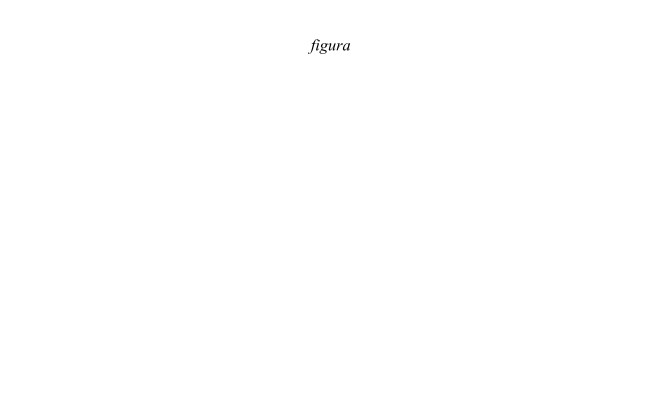
\includegraphics[width=0.98\linewidth]{figs/fig_m.jpg}		
\caption[O \gls{model} de cascata de serviços naturais]
{\textbf{---\;O \gls{casctmodel}.}
    Lorem ipsum dolor sit amet consectetur adipiscing elit. Sed ac bibendum orci. Cras erat elit, consequat vel erat ac, tincidunt pulvinar lacus. \;\textbf{a}\;---\;Sed ac bibendum orci. Cras erat elit, consequat vel erat ac, tincidunt pulvinar lacus. Pellentesque vitae consectetur quam. Interdum et malesuada fames ac ante ipsum primis in faucibus.\;\textbf{b}\;---\;Sed ac bibendum orci. Cras erat elit, consequat vel erat ac, tincidunt pulvinar lacus. Pellentesque vitae consectetur quam. Interdum et malesuada fames ac ante ipsum primis in faucibus. \;\textbf{c}\;---\;Sed ac bibendum orci. Cras erat elit, consequat vel erat ac, tincidunt pulvinar lacus. Pellentesque vitae consectetur quam. Interdum et malesuada fames ac ante ipsum primis in faucibus.
}
\label{fig:eco:cascade} 		
\end{figure}

\par Os \gls{natserv} implicados pelo conceito de \gls{natcap} trouxeram desafios tanto nas frentes teóricas quanto na prática para o desenho de políticas de \gls{sustdev}. A ideia de serviço natural, sem definições claras, torna-se pouco palpável para influenciar decisões de alocação. Em contraste, o gerenciamento de recursos não-renováveis é muito mais evidente, pois o consumo desses recursos, com sua destruição ou transformação irreversível, os torna progressivamente escassos. Sabendo que uma jazida de carvão mineral inevitavelmente se esgotará, faz sentido elaborar estratégias de diversificação energética. Por outro lado, uma floresta tropical representa um \gls{natcap} que oferece uma vasta gama de serviços, muitos dos quais são difusos e beneficiam muito além dos seus habitantes ou visitantes, em diversas escalas. Os próprios \gls{recrenew} da floresta, como a madeira ou alimentos, resultam de \gls{natservprov}, que podem ser degradados por diversas razões, como colapsos ecológicos. Para desenhar instrumentos de gestão desses \gls{natserv}, como controle, incentivos e negociações, é necessário identificá-los, mensurá-los e atribuir-lhes \textbf{\gls{econval}}. Esse é um grande desafio do novo \gls{paradigma}, ainda que existam avanços recentes.

\par Um arcabouço conceitual mais moderno para se compreender os \gls{natserv} consiste no \textbf{\gls{casctmodel}}, proposto por Haines-Young \& Potschin (2010) \cite{haines-young2010, potschin2016}. Esse \gls{model} descreve como que os serviços ecossistêmicos fluem da natureza até gerar benefícios para a sociedade em cinco etapas principais: (1) estrutura e processo; (2) função; (3) serviço; (4) benefício; e (5) valor. As primeiras três etapas pertencem à \gls{biosf}, ressaltando a importância primordial da \textbf{\gls{biophysistrc}}, como florestas e zonas úmidas, que fornecem a base para o desenvolvimento de \textbf{\gls{ecoprocess}}, como a infiltração de água e a ciclagem de nutrientes. Esses processos, por sua vez, geram \textbf{\gls{envfunc}} que podem se tornar úteis para os seres humanos. Assim, o \gls{model} enfatiza que a função ambiental de um ecos\gls{system}, ou seja, sua \textit{capacidade} de realizar algo potencialmente útil para os seres humanos, não é automaticamente um serviço natural. Apenas quando essa função é considerada \textit{benéfica} para a sociedade é que ela se torna um serviço, como a \gls{gutility} da regulação de inundações em regiões densamente povoadas. A últimas duas etapas da cascata, por outro lado, pertencem à \gls{antroposf}. O \textbf{\gls{econbenefit}}, portanto, corresponde à manifestação concreta do \gls{welbeing} derivado desse serviço natural, como uma cidade menos vulnerável aos impactos de enchentes. Mas a percepção desse bem-estar depende do contexto e das necessidades humanas específicas, o que leva à variabilidade na avaliação do seu \textbf{valor econômico}. Por exemplo, o valor varia conforme as condições de oferta e demanda: diante da explosão populacional de roedores, o \gls{econval} do \gls{natservcontrol} é muito maior do que em períodos de normalidade. Além disso, nem todos os benefícios podem ser avaliados em termos se seu \gls{exchaval}, apresentando apenas \gls{useval}, como no caso dos \gls{natservcult}, que atuam diretamente sobre o bem-estar subjetivo, sem produtos materiais intermediários.

\subsection{Classificações de serviços naturais} \label{sec:natserv:sist}

\begin{figure}[t!] 
\centering				
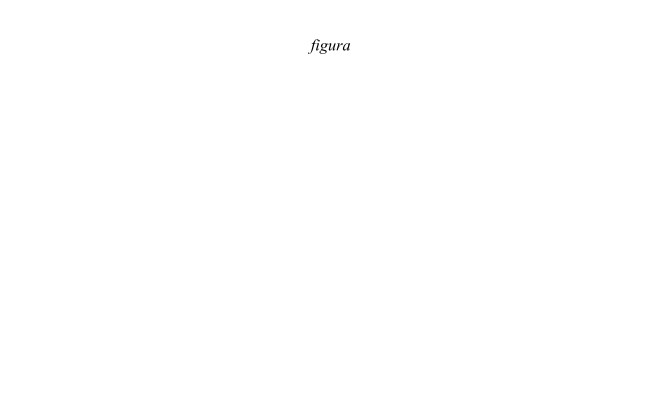
\includegraphics[width=0.98\linewidth]{figs/fig_m.jpg}		
\caption[A classificação dos Serviços Naturais]
{\textbf{---\;A classificação dos Serviços Naturais.}
    Lorem ipsum dolor sit amet consectetur adipiscing elit. Sed ac bibendum orci. Cras erat elit, consequat vel erat ac, tincidunt pulvinar lacus. \;\textbf{a}\;---\;Sed ac bibendum orci. Cras erat elit, consequat vel erat ac, tincidunt pulvinar lacus. Pellentesque vitae consectetur quam. Interdum et malesuada fames ac ante ipsum primis in faucibus.\;\textbf{b}\;---\;Sed ac bibendum orci. Cras erat elit, consequat vel erat ac, tincidunt pulvinar lacus. Pellentesque vitae consectetur quam. Interdum et malesuada fames ac ante ipsum primis in faucibus. \;\textbf{c}\;---\;Sed ac bibendum orci. Cras erat elit, consequat vel erat ac, tincidunt pulvinar lacus. Pellentesque vitae consectetur quam. Interdum et malesuada fames ac ante ipsum primis in faucibus.
}
\label{fig:eco:natserv:sist} 		
\end{figure}

\par A largada da sistematização dos \gls{natserv} foi inciada por Daily et al. (1997), especialmente no sentido de identificar e caracterizar os \gls{natserv}, mas também sobre os problemas de valoração \cite{daily1997}. Os autores definem esses serviços como \say{as condições e os processos pelos quais os ecossistemas naturais, e as espécies que os compõem, sustentam e promovem a vida humana.}. Eles trazem uma categorização pioneira, ainda que não tenham incluído detalhes sobre aspectos culturais, que separa os \textbf{\gls{natservgen}} dos \textbf{\gls{natservbiome}}. No caso dos serviços gerais, a lista inclui o \textbf{\gls{natservclim}} promovida pelos diversos ciclos biogeoquímicos (como do carbono, nitrogênio, fósforo e enxofre) e pelos ciclos da água dos sedimentos. Nessa lista, a biodiversidade é citada como um fator crítico para a estabilidade dos ecossistemas, garantindo maior resiliência a distúrbios. São mencionados também os \textbf{\gls{natservsoil}}, como a regulação do \gls{hydro_cicle}, suporte físico e fornecimento de nutrientes para plantas, além da decomposição de matéria orgânica, que recicla nutrientes e previne a proliferação de patógenos. Outros serviços gerais citados incluem o \textbf{\gls{natservpol}}, que sustenta a produção agrícola, e o \textbf{\gls{natservcontrol}}, promovido por predadores e parasitas que reduzem a necessidade de pesticidas, preservando a estabilidade da produção de alimentos. Os \gls{natserv} de biomas, por sua vez, realizam todos os serviços gerais mencionados, mas com as suas singularidades específicas em diferentes ecossistemas. Eles incluem os \gls{natserv} dos oceanos, os serviços das águas doces, os serviços das florestas e os serviços das pastagens naturais.

\par Outro marco histórico para a consolidação teórica e prática do conceito de \gls{natserv} foi o relatório \textit{Ecosystems and Human Well-being}, uma iniciativa das Nações Unidas concluída em 2005, também conhecido como o relatório da \acrfull{mea}\footnote{Avaliação Ecossistêmica do Milênio, em uma tradução livre do inglês.} \cite{MEA2005a}. Esse relatório avançou, em certa medida, o esforço de modelagem global dos \gls{natrec} divulgado em 1974 pelo Clube de Roma em \textit{Limites do crescimento} \cite{meadows1974}, trazendo dados mais detalhados sobre a distribuição e as mudanças dos ecossistemas. Na época, a avaliação destacou que aproximadamente 60\% dos \gls{natserv} estavam sendo degradados ou utilizados de forma insustentável, colocando em risco o bem-estar de populações em todo o planeta, especialmente as mais vulneráveis. Além de fornecer um dimensionamento extremamente relevante, o relatório \acrshort{mea} ajudou a consolidar a definição de \gls{natserv} como os \textit{benefícios diretos que as pessoas obtêm da natureza}. Vale destacar que o relatório \acrshort{mea} também consolidou o termo \textbf{\gls{ecoserv}}, que atualmente é o mais utilizado, embora existam variações como \textbf{\gls{envserv}}\footnote{Pessoalmente, eu prefiro a denominação \say{serviço natural}, não apenas por ser mais abrangente, mas por ser mais simples de ser compreendida pelo público leigo.}. Essa separação terminológica ainda não é totalmente clara na \gls{teoria}, mas há diferenças práticas e em marcos regulatórios. No Brasil, por exemplo, a Política Nacional de Pagamento por Serviços Ambientais faz a separação da seguinte maneira:

\begin{adjustwidth}{100pt}{0pt}
\medskip
\small 
(...)
Art. 2º Para os fins desta Lei, consideram-se:

I - ecos\gls{system}: complexo dinâmico de comunidades vegetais, animais e de microrganismos e o seu meio inorgânico que interagem como uma unidade funcional; 

II - serviços ecossistêmicos: benefícios relevantes para a sociedade gerados pelos ecossistemas, em termos de manutenção, recuperação ou melhoria das condições ambientais, (...)

III - \gls{envserv}: atividades individuais ou coletivas que favorecem a manutenção, a recuperação ou a melhoria dos serviços ecossistêmicos

-- Brasil (2021, p. 1) \cite{brasil2021}.
\medskip
\end{adjustwidth}
\noindent Apesar dessa definição oficial, o termo \say{serviço ambiental} também pode ser empregado para se referir aos benefícios obtidos de elementos naturais do ambiente construído, como em cidades. Nessa ótica, a arborização urbana, por exemplo, consistiria em uma forma de \textbf{\gls{greeninfra}} que oferece \gls{envserv}.

\par O relatório \acrshort{mea} preparou o caminho para a sistematização dos \gls{natserv} atualmente adotada pela \acrfull{cices}, que foi mencionada na seção anterior: \gls{natservprov}, \gls{natservreg} e \gls{natservcult} \cite{Haines-young2018a}. Uma quarta categoria também foi articulada pelo \acrshort{mea}, que seriam os \textbf{\gls{natservsup}}, mas na \acrshort{cices} os serviços dessa classe foram desmembrados ou mantidos conceitualmente como processos precursores dos serviços em si. A sistematização proposta pelo \acrshort{mea} e pela \acrshort{cices} adota uma abordagem oposta à de Daily et al. (1997), pois parte de uma perspectiva econômica e antropocêntrica, centrada na tipologia dos serviços, e não em sua origem na \gls{biosf}. Essa classificação orienta diretamente as decisões e avaliações relacionadas ao \gls{sustdev}, independentemente dos ecossistemas em questão. Nos serviços de provisão, a principal questão é se os materiais fornecidos pelo ecos\gls{system} estão sendo consumidos em uma taxa superior à sua capacidade de regeneração, como ocorre com a erosão dos solos agrícolas ou a pesca predatória. Nos serviços de regulação e manutenção, o foco é avaliar a capacidade do ecos\gls{system} de regular recursos, identificando até que ponto essa capacidade pode ser usada sem necessitar de medidas adicionais, como o armazenamento de água no solo para regular a disponibilidade hídrica ou a absorção de carbono pelos oceanos para mitigar o aquecimento global. Já nos serviços culturais, a questão central é identificar e valorar os benefícios imateriais que diferentes grupos obtêm do ecos\gls{system}, desde o lazer até o valor científico e educacional. Assim, essa sistematização enfatiza o aspecto econômico, facilitando a formulação de políticas para o \gls{sustdev}. Costanza (2008) sugere que isso é uma consequência inevitável da transição entre a \gls{biosf} e a \gls{antroposf}, sendo necessário se manter mais de um \gls{system} de classificação -- uns para mapear e identificar os serviços no lado da \gls{biosf} e outros para ajudar a tomada de decisão no lado da \gls{antroposf} \cite{costanza2008}.

\par A sistematização \acrshort{cices} apresenta uma estrutura hierárquica que organiza os \gls{natserv} em três níveis: as seções (nível mais alto), divisões (nível intermediário) e grupos (nível mais baixo), proporcionando uma padronização que facilita a contabilidade e o inventário ambiental. Sem um \gls{system} com esse detalhamento, seria praticamente inviável desenvolver políticas eficazes de gestão e valoração desses serviços. Com ele, projetos e ações podem ser explicitamente focadas em maximizar um ou mais \gls{natserv}. Pelo olhar hidrológico, por exemplo, a provisão de água é uma divisão dentro do serviço de provisão (código 4.2), que também abrange a provisão de biomassa e outros recursos abióticos. Essa divisão é subdividida em grupos, como a provisão de água superficial (código 4.2.1) e de água subterrânea (código 4.2.2). No caso da água superficial, as classes de serviços incluem a provisão de água potável (código 4.2.1.1), a provisão de água como insumo material (código 4.2.1.2) e a provisão de água para produção de energia (código 4.2.1.3). Esses serviços podem competir entre si, como ocorre em um reservatório que abastece uma usina hidrelétrica, onde o uso para geração de energia pode conflitar com a demanda por água potável ou industrial. No que se refere aos serviços de regulação e manutenção, a atenuação dos fluxos do \gls{hydro_cicle} na \acrshort{cices} resulta tanto de divisões bióticas (código 2.2.1.3) ou abióticas (código 5.2.1.2). A regulação biótica envolve os processos hidrológicos na escala das encostas, onde a fauna e flora influenciam a fragmentação superficial, favorecendo a infiltração. Já a regulação abiótica ocorre na escala de bacia hidrográfica, como nas planícies de inundação. Ambos os serviços demandam gestão, uma vez que podem ser prejudicados pela compactação do solo em encostas ou pela construção de diques nas planícies.

% tabela com os principais serviços relacionados com a água?

\subsection{Manifestações de valor utilitário} \label{sec:natserv:value}

\begin{figure}[t!] 
\centering				
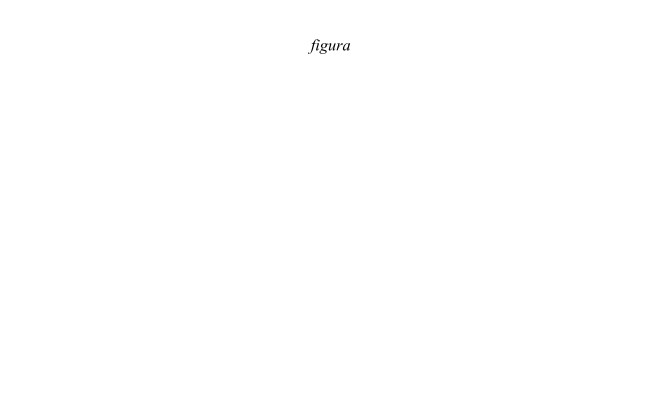
\includegraphics[width=0.98\linewidth]{figs/fig_m.jpg}		
\caption[As manifestações de valor utilitário]
{\textbf{---\;As manifestações de \gls{utilval}.}
    Lorem ipsum dolor sit amet consectetur adipiscing elit. Sed ac bibendum orci. Cras erat elit, consequat vel erat ac, tincidunt pulvinar lacus. \;\textbf{a}\;---\;Sed ac bibendum orci. Cras erat elit, consequat vel erat ac, tincidunt pulvinar lacus. Pellentesque vitae consectetur quam. Interdum et malesuada fames ac ante ipsum primis in faucibus.\;\textbf{b}\;---\;Sed ac bibendum orci. Cras erat elit, consequat vel erat ac, tincidunt pulvinar lacus. Pellentesque vitae consectetur quam. Interdum et malesuada fames ac ante ipsum primis in faucibus. \;\textbf{c}\;---\;Sed ac bibendum orci. Cras erat elit, consequat vel erat ac, tincidunt pulvinar lacus. Pellentesque vitae consectetur quam. Interdum et malesuada fames ac ante ipsum primis in faucibus.
}
\label{fig:eco:natserv:value} 		
\end{figure}

\par A valoração de \gls{natserv} envolve as duas últimas etapas do \gls{model} de cascata: a avaliação do benefício e do \gls{econval}. Para entender esse processo com profundidade, é necessário se distanciar um pouco dos aspectos práticos e retornar para questões mais teóricas. Um \textit{valor} consiste em uma métrica empregada no processo de se fazer escolhas, que sempre são orientadas por um objetivo ético supremo. Se a honestidade é um valor importante para as relações humanas, então é \textit{melhor} se relacionar com pessoas íntegras do que com pessoas mentirosas. Valorar, portanto, consiste em calcular essa métrica com base nos fundamentos éticos pré-definidos (e sermos honestos, para não sermos \textit{desvalorizados}). O valor é tido como \textit{econômico}, portanto, quando ele consiste na métrica para alocação de recursos escassos entre diferentes fins. Na \gls{ecoeco}, que se baseia no \gls{gutilitarism}, o \gls{econval} é um \textbf{\gls{utilval}} -- a \gls{gutility} ou sensação de \gls{welbeing}. Assim, apesar de todas as divergências que decorrem ao se adotar uma ontologia fisicalista, a \gls{ecoeco} se assemelha ao \gls{paradigma} econômico Neoclássico na sua dimensão ética. Ambas consideram a \gls{gutility} o \gls{ultimategoal}, ainda que a primeira reconhece o seu limite físico, e a segunda não.

\par O \gls{utilval}, contudo, não é a única forma possível de se avaliar escolhas em um contexto econômico, pois também existem formas de \textbf{\gls{intrisval}}, baseadas em direitos ou propriedades biofísicas \cite{kumar2012economics}. O \textbf{\gls{rightval}} busca corrigir o \gls{antropoc} inerente ao \gls{gutilitarism}, que, por exemplo, não garante explicitamente que outras espécies não sejam extintas, desde que isso não prejudique a contabilidade final de \gls{welbeing}. Uma alternativa a esse enfoque é o \textbf{\gls{gbiocentrism}}, que, inspirado pela ética de Kant, defende que as outras espécies possuem o direito inalienável de existir. Nesse contexto, o \textbf{\gls{impercateg}} kantiano surge como um princípio moral que deve ser seguido, independentemente das consequências utilitárias. Esse princípio ético preconiza que decisões devem ser feitas \textit{como se} fossem derivadas de uma lei \textit{universalizável}. Assim, essa lógica pode ser aplicada para se estabelecer os direitos das outras espécies, pois se não gostamos da ideia de sermos usados ou exterminados por espécies mais avançadas tecnologicamente que nós, não deveríamos fazer isso com as espécies menos avançadas \cite{daily1997}. Já o \textbf{\gls{biophyval}} utiliza métricas físicas, como energia e materiais embutidos, para decidir sobre a alocação de recursos. Esse valor é uma versão ampliada do \textbf{valor de trabalho}, identificado na economia de Karl Marx. O conceito de \textbf{\gls{ecofootprint}}, por exemplo, atribui valor com base na carga material necessária para produzir um bem ou serviço, como as pegadas de carbono e hídrica. Essas valorações, embora filosoficamente distintas, não se excluem e podem se complementar em pelo emprego de \textbf{\gls{amcrit}} ou otimização multiobjetivo. Direitos biocêntricos, por exemplo, podem funcionar como restrições sobre a extensão do utilitarismo, enquanto a análise de ciclo de vida pode alterar a sensação de satisfação ou \gls{welbeing}. Após conhecer a enorme pegada de carbono de uma viagem de avião, talvez você se disponha a pagar por uma taxa extra para compensar as emissões.

\par As possíveis manifestações do \gls{utilval} dos \gls{natserv} são sistematicamente exploradas pela iniciativa \acrfull{teeb}. Os autores dessa iniciativa definem o \textbf{\gls{tev}} como a soma de todas as formas de \gls{utilval}, organizadas em uma hierarquia de valores. Vale ressaltar que esse é um \gls{system} conceitual abrangente, aplicável tanto ao \gls{natcap} quanto ao antropogênico. Embora seja difícil e incerto obter o valor total de um dado recurso, isso geralmente não é necessário para orientar a tomada de decisão, pois os agentes econômicos costumam focar em alguns componentes específicos desse valor. Ao mesmo tempo, do ponto de vista da gestão do \gls{natcap}, o conceito de \gls{tev} é crucial para lembrar que as soluções de gestão devem considerar as perdas e ganhos entre os agentes que atuam em diferentes componentes.

\par O \gls{tev} se divide em \textbf{\gls{useval}} e \textbf{\gls{nonuseval}}. O \gls{useval}, como mencionado anteriormente, é um conceito relativamente intuitivo e bem estabelecido na \gls{gseconomics}. A \gls{marutilteo} sugere que o valor marginal de uso, ou seja, o benefício incremental obtido por unidade consumida, corresponde ao \textbf{valor de troca}, que varia conforme a oferta e demanda em mercados eficientes. Já o \gls{nonuseval} se refere à satisfação e ao bem-estar derivados de \textit{não} utilizar determinado bem ou serviço. Embora menos tangíveis, esses valores não podem ser ignorados, incluindo o \textbf{\gls{legval}}, que reflete a preocupação com a disponibilidade dos recursos para gerações futuras; o \textbf{\gls{altrval}}, que considera a equidade entre membros da geração atual; e o \textbf{\gls{existval}}, que diz respeito à satisfação obtida simplesmente pelo fato de saber que espécies e ecossistemas continuam a existir.

\par O \gls{useval} inclui tanto o \textbf{\gls{direcuseval}} quanto o \textbf{\gls{indirectuseval}}. O \gls{direcuseval} refere-se à interação explícita com o recurso, seja ele um serviço natural ou um bem de consumo convencional. Esse uso direto pode ser \textbf{\gls{useconsum}} ou \textbf{\gls{usenonconsun}}. O uso \gls{useconsum} envolve a transformação irreversível do recurso, que é o caso de todos os recursos do tipo estoque-fluxo. O uso \gls{usenonconsun}, por outro lado, relaciona-se mais com os recursos do tipo fundo-serviço, que não são transformados. Ao ir ao cinema, a pipoca tem um \gls{direcuseval} e \gls{useconsum}, mas o filme tem \gls{direcuseval} \gls{usenonconsun}. No contexto do \gls{natcap}, os \gls{natservprov} disponibilizam recursos com \gls{direcuseval} \gls{useconsum}, enquanto que os \gls{natservcult} exibem \gls{direcuseval} \gls{usenonconsun}. A água de um rio que abastece uma cidade, por exemplo, possui \gls{direcuseval} \gls{useconsum}, pois a água é transformada nesse processo. Mas as práticas de esportes náuticos nesse mesmo rio consiste apresenta \gls{direcuseval} \gls{usenonconsun}. O \gls{indirectuseval}, por outro lado, refere-se a interações menos explícitas com o recurso, onde o valor se manifesta por meio de processos intermediários que muitas vezes não são imediatamente visíveis. Usando o exemplo do cinema, dificilmente interagimos diretamente com a equipe de limpeza, mas a manutenção do ambiente limpo melhora nossa experiência. Nessa linha, no contexto do \gls{natcap}, o uso indireto está associado a \gls{natservreg}. A polinização realizada por insetos, por exemplo, é essencial para a agricultura, mas esse serviço não envolve uma interação direta entre o consumidor dos alimentos e os polinizadores. Da mesma forma, a infiltração de água nas encostas beneficia os usuários a jusante, que se beneficiam da disponibilidade de água limpa, mesmo sem interagir diretamente com o processo natural.

\par O \gls{direcuseval} e o \gls{indirectuseval} são ambos formas de \gls{useval} \textit{no presente}. No entanto, os autores da \acrshort{teeb} também destacam uma forma de \textbf{\gls{futuseval}}, conhecida como \textbf{\gls{optionval}}. Esse valor, no contexto do \gls{natcap}, está fortemente relacionado à capacidade dos ecossistemas de se manterem resilientes e se recuperarem de perturbações. Contudo, essa resiliência tem limites e pode ser comprometida quando o ecos\gls{system} é submetido a uma perturbação muito intensa, ultrapassando um \textbf{\gls{tippingpoint}}. A partir desse limiar crítico, o atrator do \gls{system} migra para uma nova região, que pode ser estável ou instável, resultando na perda ou degradação significativa dos \gls{natserv} previamente disponíveis. Um exemplo de mudança de regime estável-estável é a introdução de espécies invasoras, que alteram rapidamente o equilíbrio ecológico, reduzindo a biodiversidade. Nessa situação, a restauração do ecos\gls{system} original torna-se extremamente onerosa, pois o atrator do \gls{system} encontra-se em outro ponto ou região de estabilidade. Já uma mudança de regime estável-instável ocorre quando a erosão do solo progride de pequenos sulcos para grandes ravinas e voçorocas, com fortes retroações positivas que intensificam o processo de erosão cada vez mais. O \gls{optionval} reflete a \textbf{\gls{riskaversv}} de mudanças de regime no \gls{system}, que acarretariam custos exorbitantes. Nesse contexto, a \gls{uncert-episteme} — a falta de conhecimento sobre o \gls{system} — torna-se um fator crucial na avaliação desse valor, aumentando à medida que a ignorância sobre o comportamento do \gls{system} é reconhecida. O \gls{futuseval}, portanto, está diretamente ligado ao \textbf{\gls{precauprinci}}, que orienta que, em condições de alta incerteza sobre os pontos de não-retorno, as políticas devem ser guiadas por salvaguardas conservadoras.

\subsection{Métodos de valoração}

\par A determinação de cada componente do \gls{tev} envolve o uso de uma variedade de métodos, que avançam por estratégias incrementais, de acordo com as informações de \gls{useval} marginal (preços) disponíveis. É claro que limitações técnicas, metodológicas e de incerteza dos métodos de valoração aumentam conforme a escassez de informações disponíveis. Quando os \gls{natserv} estão fortemente vinculados a mercados reais, pode-se aplicar técnicas de \textbf{\gls{valuadm}}. Em situações em que os \gls{natserv} tem uma relação indireta com mercados reais, busca-se informações em mercados reais paralelos pela aplicação de técnicas de \textbf{\gls{valuarevpref}}. Por fim, diante da ausência completa de um mercado real ou paralelo, as alternativas de valoração lançam mão de técnicas de \textbf{\gls{valuastatpref}}, estimando o valor em mercados hipotéticos.

\par No caso mais básico, a \gls{valuadm} identifica as transações de mercado que estão vinculadas diretamente aos \gls{natserv}. Esse método se divide em três categorias principais: \textbf{\gls{valuaprice}}, \textbf{\gls{valuacost}} e \textbf{\gls{valuafuncprod}}. A \gls{valuaprice} de mercado relaciona-se com os \gls{natservprov} cujos produtos são negociados em mercados. A abordagem é a mais direta possível: o \gls{useval} marginal, direto e \gls{useconsum}, é o \gls{gprice} de mercado, que pode ser corrigido para se remover eventuais distorções. As abordagens baseadas em custos, mais associadas aos \gls{natservreg}, focam na estimativa dos gastos necessários para recriar os benefícios dos \gls{natserv} por meios artificiais. Entre essas técnicas estão o \textbf{\gls{valuaavoid}}, que considera os custos de produção que seriam incorridos na ausência dos \gls{natserv}; o \textbf{\gls{valuarepo}}, que estima o valor necessário para substituir o serviço em si por tecnologias artificiais; e \textbf{\gls{valuarest}}, que avalia os gastos para mitigar a perda dos \gls{natserv} ou restaurá-los. Por sua vez, as abordagens baseadas em funções de produção são as abordagens mais integradas possíveis dessa categoria, quando existe conhecimento suficiente pra fazer a conexão causal do desempenho dos \gls{natserv} sobre a produção de um bem ou serviço negociado em mercados. 

\par Na situação intermediária, as técnicas de preferência revelada baseiam-se na observação das escolhas individuais em mercados existentes que estão relacionados indiretamente ao serviço natural em questão. Ou seja, os agentes econômicos \textit{revelam} a \gls{gutility} do serviço por meio de suas escolhas. Os autores da \acrshort{teeb} ressaltam que as principais metodologias dentro desse escopo são o \textbf{\gls{valuatravcost}} e o \textbf{\gls{valuahedonpric}}, ambos fortemente relacionados com \gls{natservcult}, valores com uso direto e \gls{usenonconsun}. A estimativa de custos de viagem é essencial para valorar os serviços culturais relacionados com atividades turísticas e de lazer, que inclui despesas diretas e o \gls{opcost} do tempo. Assim, o valor de uma mudança na qualidade ou quantidade de um local recreativo pode ser inferido a partir da função de demanda estimada para as visitas. Por outro lado, a precificação hedônica utiliza informações sobre a demanda implícita por um atributo ambiental embutido em recursos que são negociados em mercados. Um exemplo típico desse \textit{valor agregado} é a beleza cênica altamente valorizada nos preços de imóveis com vistas para paisagens naturais. A instalação de turbinas eólicas e outros aspectos de poluição visual na paisagem podem causar a perda desse esse serviço natural cultural, fato que se manifesta pela desvalorização de imóveis, por exemplo.

\par Por fim, na ausência de informações disponíveis em mercados, as abordagens de preferência declarada simulam um mercado hipotético para os \gls{natserv} por meio de pesquisas que consideram mudanças na provisão desses serviços. Essas técnicas podem estimar tanto valores de uso quanto de não-uso, como o valor da existência ou \gls{legval}. Entre as técnicas disponíveis está o \textbf{\gls{valuacontg}}, que utiliza questionários para se inferir dos agentes econômicos a sua disposição a pagar por melhorias em um serviço natural ou a disposição a aceitar a degradação em um serviço natural, sendo duas faces da mesma moeda. Uma forma mais complexa consiste no método de \textbf{\gls{valuachoice}}, quando os respondentes dos questionários são submetidos a uma rede de escolhas possíveis, sinalizando melhor as relações declaradas de perdas e ganhos. Uma avaliação ainda mais robusta inclui a \textbf{\gls{valuagroups}}, quando diferentes grupos de agentes econômicos participam em um processo plural para deliberar o valor de um dado serviço ou recurso natural. Esse processo viabiliza, com abordagens multi-critério, a integração com outras métricas de valor e sistemas éticos mencionados acima.

\section{Serviços naturais hidrológicos} \label{chap:ecoeco:watersheds}

\begin{figure}[t!] 
\centering				
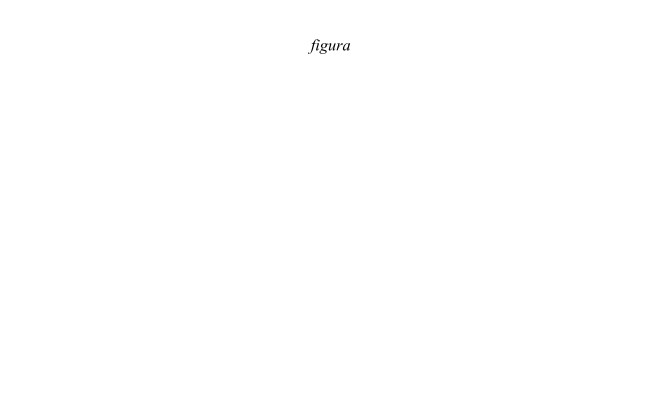
\includegraphics[width=0.98\linewidth]{figs/fig_m.jpg}		
\caption[Lorem ipsum dolor sit amet]
{\textbf{---\;Lorem ipsum dolor sit amet.}
    Lorem ipsum dolor sit amet consectetur adipiscing elit. Sed ac bibendum orci. Cras erat elit, consequat vel erat ac, tincidunt pulvinar lacus. \;\textbf{a}\;---\;Sed ac bibendum orci. Cras erat elit, consequat vel erat ac, tincidunt pulvinar lacus. Pellentesque vitae consectetur quam. Interdum et malesuada fames ac ante ipsum primis in faucibus.\;\textbf{b}\;---\;Sed ac bibendum orci. Cras erat elit, consequat vel erat ac, tincidunt pulvinar lacus. Pellentesque vitae consectetur quam. Interdum et malesuada fames ac ante ipsum primis in faucibus. \;\textbf{c}\;---\;Sed ac bibendum orci. Cras erat elit, consequat vel erat ac, tincidunt pulvinar lacus. Pellentesque vitae consectetur quam. Interdum et malesuada fames ac ante ipsum primis in faucibus.
}
\label{fig:eco:watersheds} 		
\end{figure}

\subsection{Sec1}

Conceitos importantes:
\begin{itemize}
    \item         escala operacional
    \item valoração
    \item comando e controle: zoneamento 
    \item incentivos: pagamentos
    \item negociações: mercado
    \item mapeamento de processos com modelos
\end{itemize} 

\par Com o advento da Economia Ecológica e seu conceito de capital natural, novas perspectivas surgem para o enquadramento do \textbf{gerenciamento integrado de recursos hídricos}, que, como paradigma de gestão e planejamento de bacias hidrográficas, visa garantir a \textbf{segurança hídrica}. As Nações Unidas definem segurança hídrica como a capacidade de uma população de assegurar o acesso sustentável a quantidades adequadas de água de qualidade aceitável, necessárias para sustentar meios de subsistência, bem-estar humano e desenvolvimento socioeconômico, além de proteger contra poluição e desastres relacionados à água, e preservar ecossistemas em um contexto de paz e estabilidade política [todo:cite cassin]. Essa noção conceitual é complexa, e abrange quatro elementos centrais: água potável e bem-estar humano; ecossistemas; riscos relacionados à água e mudanças climáticas, e; atividades econômicas e desenvolvimento sustentável. Na prática, porém, garantir a segurança hídrica implica a necessidade de planejar e gerir programas, projetos e ações que, dentro dos contextos socioeconômicos e geopolíticos, garantam a qualidade, a quantidade e a regularidade da água em condições suficientes para atender demandas de múltiplos usuários, além de mitigar os riscos humanos associados a eventos extremos, como grandes enchentes e deslizamentos. 

\par Os usuários de água em uma bacia hidrográfica consistem em diferentes agentes econômicos, que vão desde comunidades tradicionais, passando por companhias de abastecimento de água até setores econômicos como agricultura, indústria e produção de energia. Sob o paradigma ecológico-econômico, a água deixa de ser vista somente como um fator de produção para esses agentes econômicos e passa a ser reconhecida como um recurso natural comum fornecido pelo capital natural da bacia hidrográfica. Nessa ótica, torna-se claro que a alocação da água para os diferentes usos envolve, na verdade, o consumo de uma série de serviços naturais fornecidos pelos ecossistemas da bacia, denominados de \textbf{serviços naturais hidrológicos}. Smith et al. (2006) demonstram que esses serviços vão além da simples provisão de água, incluindo também a provisão de alimentos, a regulação dos fluxos de água e sedimentos, a qualidade da água, a mitigação de riscos hidrológicos e diversos serviços naturais culturais\cite{Smith2006a}.

{\renewcommand{\arraystretch}{1.5}
\begin{table}[t!]
    \centering	
    \tiny
    \sffamily
    \rowcolors{2}{white}{rowgray}
    \begin{tabular}{ 
        >{\raggedright\arraybackslash}m{1.5cm} 
        >{\raggedright\arraybackslash}m{2.5cm}  
        >{\raggedright\arraybackslash}m{3.0cm}  
        >{\raggedright\arraybackslash}m{2.5cm}
        >{\raggedright\arraybackslash}m{2.5cm}
    }
    \toprule 
    \textbf{Service section} & \textbf{Watershed services} & \textbf{Service attributes} & \textbf{State indicator} & \textbf{Sustainable use indicator} \\ 
    \midrule 
    \textbf{Provision} & Water supply & Precipitation, infiltration, soil retention, percolation, streamflow, groundwater flow, biotic and abiotic effects on water quality & Water storage capacity (m³/m²), Pollutant concentrations & Discharge (m³/year) \\ 
    
    \cline{2-5} 
     & Food provision & Crop, fruit, livestock production, edible plants and animals (e.g., fish, algae, invertebrates) & Agricultural water use (m³/ha), Fish stock (kg/m³) & Maximum sustainable water use for irrigation (m³/year), Net productivity (kg/ha/year) \\ 
    
    \cline{2-5}
     & Non-food goods & Production of raw materials (e.g., timber, reeds), production of medicines & Amounts available (kg/ha/year) & Maximum sustainable harvest (kg/ha/year) \\ 
    
    \cline{2-5} & Hydro-electric power & Flow for energy generation & Storage capacity of riverbeds and lakes (m³/m²), Slope (degree), Elevation (m) & Maximum sustainable energy production (kWh/year) \\ 
    
    \textbf{Regulation} & Regulation of water flows & Retention of rainfall and release (especially by forests and wetlands), Water storage by rivers, lakes, and wetlands, Groundwater recharge and discharge & Infiltration capacity (mm/h), Water storage capacity of soils (m³/m²) & Baseflow volume (m³/year) \\ 
    
    \cline{2-5}
    & Hazard mitigation & Reduced flood peaks and storm damage, Coastal protection, Slope stability & Maximum natural water storage capacity (m³/m²) & Size (km²) and economic value (US\$/km²/year) are protected from flooding \\ 
    
    \cline{2-5}
    & Control of soil erosion and sedimentation & Protection of soil by vegetation and soil biota & Infiltration capacity (mm/h), Slope length (m), Barren land (\%) & Soil loss (kg/ha/year), Sediment storage (kg/m²/year) \\ 
    
    \cline{2-5}
    & Water purification & Reduced siltation of streams and lakes, Nutrient uptake and release by ecosystems, Removal of organic matter, salts, pollutants & Nitrogen amount (kg/ha), Total dissolved solids (kg/m²), Electric conductivity (\(\mu\)S/cm) & Denitrification (kg/ha/year) \\ 
    
    \cline{2-5}
    & Wildlife habitat & Wildlife and nursery habitats & Resident and endemic species (number), Surface area per ecosystem type (ha) & 
    Increase or decline in species population size (number) \\ 
    
    \cline{2-5} 
    & Environmental flows & Maintenance of river flow regime & Area of critical habitats (ha), Discharge for each season (m³/day) & Fish species and population, Total fish catch (t/year) \\ 
    
    \textbf{Cultural} & Aesthetic and recreational services & Landscape quality and features, Recreational value & Stated appreciation, Recreational value (e.g., entrance fees, US\$/visit) & Houses on lakeshore (number/km), Visitors (number/year) \\ 
    
    \cline{2-5} 
    & Heritage and identity & Landscape features or species & Cultural significance and sense of belonging & Visitors (number/year) \\ 
    
    \cline{2-5} 
    & Spiritual and artistic inspiration & Inspirational value of landscape features and species & Books and paintings using watershed as inspiration & Pilgrims (number/year) \\ 
    
    \bottomrule
    \end{tabular}
    \caption[Os serviços naturais hidrológicos]{
        \textbf{Serviços naturais hidrológicos}\; --- \;Relação dos serviços naturais hidrológicos, principais atributos, indicadores de estado e indicadores de uso sustentável. Adaptado de Smith et \textit{al.} (2006) \cite{Smith2006a}.}
    \label{tbl:nbs}
\end{table}
}

\par A extensão espacial dos serviços naturais hidrológicos está diretamente vinculada à bacia hidrográfica, o que os diferencia de outros serviços ecossistêmicos, como a regulação climática, que ocorre em escala global, ou os serviços dos biomas, que se manifestam em áreas muito mais amplas. A dinâmica de montante para jusante nas bacias hidrográficas gera uma cadeia causal de respostas hidrológicas, que se traduz economicamente em externalidades, tanto positivas quanto negativas. Esses efeitos variam conforme o estado de conservação dos serviços naturais nas áreas de montante e o uso desses serviços nas regiões de jusante. Seguindo o modelo de cascata, fica claro que os serviços hidrológicos são frutos da interação entre a vegetação, o solo, a geologia e a topografia da bacia hidrográfica. Como discutido no Capítulo \ref{chap:hydrology}, esses serviços são, em grande parte, resultantes dos processos hidrológicos que ocorrem nas encostas e nas bacias de ordem zero. Em bacias maiores, esses serviços podem se manifestar por meio de eventos como a inundação de planícies e o funcionamento ecológico das áreas úmidas, que também contribuem na regulação do ciclo hidrológico. Reconhecer esse fluxo de externalidades cria a oportunidade de gerenciar o capital natural de forma a mitigar o problema do livre acesso e evitar a tragédia dos comuns. As políticas de gestão, nesse sentido, devem estabelecer conexões estratégicas entre os usuários da água nas áreas de jusante e os agentes econômicos responsáveis pela conservação e manejo nas encostas de montante. Com isso, objetiva-se manter o uso da bacia hidrográfica dentro do limite econômico postulado pela Economia Ecológica.

\par Em um mundo de urbanização acelerada, a segurança hídrica depende da gestão dos mananciais urbanos. Nessa linha, o relatório do Banco Mundial de Dudley et al. (2003) \cite{Dudley2003a} consolidou a importância da gestão dos serviços naturais hidrológicos em áreas de mananciais, destacando que florestas bem manejadas e áreas protegidas podem melhorar tanto a qualidade quanto a quantidade de água fornecida. O estudo mostrou que florestas naturais, especialmente as bem conservadas, oferecem água de maior qualidade, com menos sedimentos e poluentes, em comparação a outras áreas de captação. Além disso, florestas tropicais nativas e maduras podem aumentar a vazão de água, embora florestas jovens e plantações exóticas possam reduzir esse fluxo. O relatório também revelou que cerca de um terço (33 de 105) das maiores cidades do mundo obtêm água diretamente de áreas protegidas, enquanto outras cinco dependem de bacias hidrográficas distantes que incluem áreas protegidas, e pelo menos oito cidades obtêm água de florestas manejadas com foco no abastecimento hídrico. Apesar dos benefícios dessas áreas para o abastecimento urbano e a biodiversidade, o valor econômico dos serviços hidrológicos ainda é subestimado. O relatório propôs a criação de mecanismos financeiros, como a cobrança de taxas de usuários, para ajudar a custear a proteção e manejo dessas áreas, o que hoje se enquadra nos Esquemas de Pagamento por Serviços Ambientais (mais detalhes adiante).

\par A maximização da segurança hídrica, portanto, passa a ser concebida através da integração entre o capital antropogênico e o capital natural. As cidades, por exemplo, dependem da \textbf{infraestrutura cinza} para obter água potável, como barragens de armazenamento, estações de bombeamento e tratamento, entre outros. No entanto, a vegetação e o solo presentes na bacia hidrográfica, acima do ponto de captação, funcionam como uma \textbf{infraestrutura verde}, que atua de forma complementar ao reduzir a intensidade de enxurradas nas encostas, um processo de resposta rápida com alto potencial erosivo. Esse arranjo, que alia infraestruturas verdes e cinzas, vem sendo cada vez mais enquadrado pelo conceito de Soluções Baseadas na Natureza (SBN), práticas que se inspiram ou fazem uso direto de processos naturais para melhorar a gestão da água, a produção de alimentos e a conservação da biodiversidade (WWAP/UN-WATER, 2018; SONNEVELD et al., 2018) [todo:cite]. A ideia subjacente às SBN integra conceitos já estabelecidos, como a engenharia ecológica, manejo conservacionista do solo e abordagens de gestão ambiental. Além disso, está alinhada aos princípios da Economia Ecológica, que reconhece a importância central do capital natural para o desenvolvimento sustentável [todo:cite Nesshöver et al. (2017)].

\par O diferencial do conceito das Soluções Baseadas na Natureza (SBN) está no fato de que ele não necessariamente requer a preservação de um capital natural prístino e intocável, como a vegetação nativa, mas se expande ao se inspirar nos processos naturais, permitindo projetar uma transição ecológica que favoreça a \textit{reprodução} desses processos, mesmo em paisagens modificadas. Por exemplo, uma lavoura que adota técnicas de plantio direto com terraços e cordões de infiltração reproduz uma estrutura biofísica análoga aos processos de infiltração observados em áreas de floresta nativa. Assim, as SBN facilitam a restauração de ecossistemas e a recuperação de serviços ambientais ao integrar práticas que imitam funções ecológicas essenciais em ambientes manejados. A silvicultura ou a agrofloresta, com o plantio de árvores exóticas não invasoras, também pode contribuir para a recuperação de solos degradados, regenerando o horizonte orgânico e preparando o solo para a regeneração da mata nativa em etapas subsequentes. Dessa forma, as SBN promovem uma transição gradual e sustentável para a regeneração ecológica, sem depender exclusivamente de ecossistemas naturais intactos.

{\renewcommand{\arraystretch}{1.5}
\begin{table}[t!]
    \centering	
    \tiny
    \sffamily
    \rowcolors{2}{white}{rowgray}
    \begin{tabular}{ 
 >{\raggedright\arraybackslash}m{2.5cm}  
 >{\raggedright\arraybackslash}m{3.5cm}  
 >{\raggedright\arraybackslash}m{1.0cm}
 >{\raggedright\arraybackslash}m{1.0cm}
 >{\raggedright\arraybackslash}m{1.0cm}
 >{\raggedright\arraybackslash}m{2.5cm}}
    \toprule 
    \textbf{Water management issue/natural service} & \textbf{Green Infrastructure solution} & \textbf{Watershed} & \textbf{Floodplain} & \textbf{Urban} & \textbf{Corresponding Grey Infrastructure solution}\\ 
    \midrule
    \textbf{Water supply (flow regulation)} & Re/afforestation and forest conservation & x &  &  & Dams and groundwater pumping \\
    \cline{2-5}
    & Reconnecting rivers to floodplains & x & x &  & Water distribution systems \\
    \cline{2-5}
    & Wetlands restoration/conservation & x & x & x &  \\
    \cline{2-5}
    & Constructing wetlands &  & x & x &  \\
    \cline{2-5}
    & Water harvesting &  &  & x &  \\
    \cline{2-5}
    & Bioretention and infiltration & x &  & x &  \\
    \cline{2-5}
    & Permeable pavements &  &  & x &  \\
    
    \textbf{Water purification (quality regulation)}& Re/afforestation and forest conservation & x &  &  & Water treatment plant \\
    \cline{2-5}
    & Reconnecting rivers to floodplains & x & x &  &  \\
    \cline{2-5}
    & Riparian buffers & x &  &  &  \\
    \cline{2-5}
    & Wetlands restoration/conservation & x & x & x &  \\
    \cline{2-5}
    & Constructing wetlands &  & x & x &  \\
    \cline{2-5}
    & Bioretention and infiltration & x &  & x &  \\
    \cline{2-5}
    & Permeable pavements &  &  & x &  \\
    
    \textbf{Erosion control (quality regulation)}& Re/afforestation and forest conservation & x &  &  & Reinforcement of slopes \\
    \cline{2-5}
    & Riparian buffers & x &  &  &  \\
    \cline{2-5}
    & Reconnecting rivers to floodplains & x & x &  &  \\
    \cline{2-5}
    & Wetlands restoration/conservation & x & x & x &  \\
    \cline{2-5}
    & Constructing wetlands &  & x & x &  \\
    
    \textbf{Water temperature control (quality regulation)}& Re/afforestation and forest conservation & x &  &  & Dams \\
    \cline{2-5}
    & Riparian buffers & x &  &  &  \\
    \cline{2-5}
    & Reconnecting rivers to floodplains & x & x &  &  \\
    \cline{2-5}
    & Wetlands restoration/conservation & x & x & x &  \\
    \cline{2-5}
    & Constructing wetlands &  & x & x &  \\
    \cline{2-5}
    & Green spaces (shading of water ways) &  &  & x &  \\
    
    \textbf{Biological control (quality regulation)}& Re/afforestation and forest conservation & x &  &  & Water treatment plant \\
    \cline{2-5}
    & Riparian buffers & x &  &  &  \\
    \cline{2-5}
    & Reconnecting rivers to floodplains & x & x &  &  \\
    \cline{2-5}
    & Wetlands restoration/conservation & x & x & x &  \\
    \cline{2-5}
    & Constructing wetlands &  & x & x &  \\
    
    \textbf{Riverine flood control (disturbance regulation)}& Re/afforestation and forest conservation & x &  &  & Dams and levees \\
    \cline{2-5}
    & Riparian buffers & x &  &  &  \\
    \cline{2-5}
    & Reconnecting rivers to floodplains & x & x &  &  \\
    \cline{2-5}
    & Wetlands restoration/conservation & x & x & x &  \\
    \cline{2-5}
    & Constructing wetlands &  & x & x &  \\
    \cline{2-5}
    & Establishing flood bypasses &  & x &  &  \\
    
    \textbf{Urban stormwater (disturbance regulation)}& Green roofs &  &  & x & Urban stormwater infrastructure  \\
    \cline{2-5}
    & Bioretention and infiltration &  &  & x & \\
    \cline{2-5}
    & Water harvesting &  &  & x &  \\
    \cline{2-5}
    & Permeable pavements &  &  & x &  \\
    
    \bottomrule
    \end{tabular}
    \caption[Green infrastructure for hydrological natural services]{
    \textbf{Green infrastructure solution for enhancing hydrological natural services}\; --- \;Systematized relationship by Cassin et \textit{al.} (2021) \cite{cassin2021} between natural hydrological services, green infrastructure, application scales (watershed, floodplain, or cities), and the corresponding grey infrastructure solution.
    }
    \label{tbl:nbs}
\end{table}
}

\cite{Smith2006a}



\par Cras erat elit, consequat vel erat ac, tincidunt pulvinar lacus. Pellentesque vitae consectetur quam. Interdum et malesuada fames ac ante ipsum primis in faucibus. Curabitur at mollis eros. Integer ornare erat neque, id finibus velit ultrices in. Suspendisse dapibus tortor eget lorem pretium venenatis. Cras erat elit, consequat vel erat ac, tincidunt pulvinar lacus. Pellentesque vitae consectetur quam. Interdum et malesuada fames ac ante ipsum primis in faucibus. Curabitur at mollis eros. Integer ornare erat neque, id finibus velit ultrices in. Suspendisse dapibus tortor eget lorem pretium venenatis. Cras erat elit, consequat vel erat ac, tincidunt pulvinar lacus. Pellentesque vitae consectetur quam. Interdum et malesuada fames ac ante ipsum primis in faucibus. Curabitur at mollis eros. Integer ornare erat neque, id finibus velit ultrices in. Suspendisse dapibus tortor eget lorem pretium venenatis.

\par Cras erat elit, consequat vel erat ac, tincidunt pulvinar lacus. Pellentesque vitae consectetur quam. Interdum et malesuada fames ac ante ipsum primis in faucibus. Curabitur at mollis eros. Integer ornare erat neque, id finibus velit ultrices in. Suspendisse dapibus tortor eget lorem pretium venenatis. Cras erat elit, consequat vel erat ac, tincidunt pulvinar lacus. Pellentesque vitae consectetur quam. Interdum et malesuada fames ac ante ipsum primis in faucibus. Curabitur at mollis eros. Integer ornare erat neque, id finibus velit ultrices in. Suspendisse dapibus tortor eget lorem pretium venenatis. Cras erat elit, consequat vel erat ac, tincidunt pulvinar lacus. Pellentesque vitae consectetur quam. Interdum et malesuada fames ac ante ipsum primis in faucibus. Curabitur at mollis eros. Integer ornare erat neque, id finibus velit ultrices in. Suspendisse dapibus tortor eget lorem pretium venenatis.

\par Cras erat elit, consequat vel erat ac, tincidunt pulvinar lacus. Pellentesque vitae consectetur quam. Interdum et malesuada fames ac ante ipsum primis in faucibus. Curabitur at mollis eros. Integer ornare erat neque, id finibus velit ultrices in. Suspendisse dapibus tortor eget lorem pretium venenatis. Cras erat elit, consequat vel erat ac, tincidunt pulvinar lacus. Pellentesque vitae consectetur quam. Interdum et malesuada fames ac ante ipsum primis in faucibus. Curabitur at mollis eros. Integer ornare erat neque, id finibus velit ultrices in. Suspendisse dapibus tortor eget lorem pretium venenatis. Cras erat elit, consequat vel erat ac, tincidunt pulvinar lacus. Pellentesque vitae consectetur quam. Interdum et malesuada fames ac ante ipsum primis in faucibus. Curabitur at mollis eros. Integer ornare erat neque, id finibus velit ultrices in. Suspendisse dapibus tortor eget lorem pretium venenatis.

\par Cras erat elit, consequat vel erat ac, tincidunt pulvinar lacus. Pellentesque vitae consectetur quam. Interdum et malesuada fames ac ante ipsum primis in faucibus. Curabitur at mollis eros. Integer ornare erat neque, id finibus velit ultrices in. Suspendisse dapibus tortor eget lorem pretium venenatis. Cras erat elit, consequat vel erat ac, tincidunt pulvinar lacus. Pellentesque vitae consectetur quam. Interdum et malesuada fames ac ante ipsum primis in faucibus. Curabitur at mollis eros. Integer ornare erat neque, id finibus velit ultrices in. Suspendisse dapibus tortor eget lorem pretium venenatis. Cras erat elit, consequat vel erat ac, tincidunt pulvinar lacus. Pellentesque vitae consectetur quam. Interdum et malesuada fames ac ante ipsum primis in faucibus. Curabitur at mollis eros. Integer ornare erat neque, id finibus velit ultrices in. Suspendisse dapibus tortor eget lorem pretium venenatis.

\par Cras erat elit, consequat vel erat ac, tincidunt pulvinar lacus. Pellentesque vitae consectetur quam. Interdum et malesuada fames ac ante ipsum primis in faucibus. Curabitur at mollis eros. Integer ornare erat neque, id finibus velit ultrices in. Suspendisse dapibus tortor eget lorem pretium venenatis. Cras erat elit, consequat vel erat ac, tincidunt pulvinar lacus. Pellentesque vitae consectetur quam. Interdum et malesuada fames ac ante ipsum primis in faucibus. Curabitur at mollis eros. Integer ornare erat neque, id finibus velit ultrices in. Suspendisse dapibus tortor eget lorem pretium venenatis. Cras erat elit, consequat vel erat ac, tincidunt pulvinar lacus. Pellentesque vitae consectetur quam. Interdum et malesuada fames ac ante ipsum primis in faucibus. Curabitur at mollis eros. Integer ornare erat neque, id finibus velit ultrices in. Suspendisse dapibus tortor eget lorem pretium venenatis.

\par Cras erat elit, consequat vel erat ac, tincidunt pulvinar lacus. Pellentesque vitae consectetur quam. Interdum et malesuada fames ac ante ipsum primis in faucibus. Curabitur at mollis eros. Integer ornare erat neque, id finibus velit ultrices in. Suspendisse dapibus tortor eget lorem pretium venenatis. Cras erat elit, consequat vel erat ac, tincidunt pulvinar lacus. Pellentesque vitae consectetur quam. Interdum et malesuada fames ac ante ipsum primis in faucibus. Curabitur at mollis eros. Integer ornare erat neque, id finibus velit ultrices in. Suspendisse dapibus tortor eget lorem pretium venenatis. Cras erat elit, consequat vel erat ac, tincidunt pulvinar lacus. Pellentesque vitae consectetur quam. Interdum et malesuada fames ac ante ipsum primis in faucibus. Curabitur at mollis eros. Integer ornare erat neque, id finibus velit ultrices in. Suspendisse dapibus tortor eget lorem pretium venenatis.

\par Cras erat elit, consequat vel erat ac, tincidunt pulvinar lacus. Pellentesque vitae consectetur quam. Interdum et malesuada fames ac ante ipsum primis in faucibus. Curabitur at mollis eros. Integer ornare erat neque, id finibus velit ultrices in. Suspendisse dapibus tortor eget lorem pretium venenatis. Cras erat elit, consequat vel erat ac, tincidunt pulvinar lacus. Pellentesque vitae consectetur quam. Interdum et malesuada fames ac ante ipsum primis in faucibus. Curabitur at mollis eros. Integer ornare erat neque, id finibus velit ultrices in. Suspendisse dapibus tortor eget lorem pretium venenatis. Cras erat elit, consequat vel erat ac, tincidunt pulvinar lacus. Pellentesque vitae consectetur quam. Interdum et malesuada fames ac ante ipsum primis in faucibus. Curabitur at mollis eros. Integer ornare erat neque, id finibus velit ultrices in. Suspendisse dapibus tortor eget lorem pretium venenatis.

\subsection{Identificação}

\par Cras erat elit, consequat vel erat ac, tincidunt pulvinar lacus. Pellentesque vitae consectetur quam. Interdum et malesuada fames ac ante ipsum primis in faucibus. Curabitur at mollis eros. Integer ornare erat neque, id finibus velit ultrices in. Suspendisse dapibus tortor eget lorem pretium venenatis. Cras erat elit, consequat vel erat ac, tincidunt pulvinar lacus. Pellentesque vitae consectetur quam. Interdum et malesuada fames ac ante ipsum primis in faucibus. Curabitur at mollis eros. Integer ornare erat neque, id finibus velit ultrices in. Suspendisse dapibus tortor eget lorem pretium venenatis. Cras erat elit, consequat vel erat ac, tincidunt pulvinar lacus. Pellentesque vitae consectetur quam. Interdum et malesuada fames ac ante ipsum primis in faucibus. Curabitur at mollis eros. Integer ornare erat neque, id finibus velit ultrices in. Suspendisse dapibus tortor eget lorem pretium venenatis.

\par Cras erat elit, consequat vel erat ac, tincidunt pulvinar lacus. Pellentesque vitae consectetur quam. Interdum et malesuada fames ac ante ipsum primis in faucibus. Curabitur at mollis eros. Integer ornare erat neque, id finibus velit ultrices in. Suspendisse dapibus tortor eget lorem pretium venenatis. Cras erat elit, consequat vel erat ac, tincidunt pulvinar lacus. Pellentesque vitae consectetur quam. Interdum et malesuada fames ac ante ipsum primis in faucibus. Curabitur at mollis eros. Integer ornare erat neque, id finibus velit ultrices in. Suspendisse dapibus tortor eget lorem pretium venenatis. Cras erat elit, consequat vel erat ac, tincidunt pulvinar lacus. Pellentesque vitae consectetur quam. Interdum et malesuada fames ac ante ipsum primis in faucibus. Curabitur at mollis eros. Integer ornare erat neque, id finibus velit ultrices in. Suspendisse dapibus tortor eget lorem pretium venenatis.

\par Cras erat elit, consequat vel erat ac, tincidunt pulvinar lacus. Pellentesque vitae consectetur quam. Interdum et malesuada fames ac ante ipsum primis in faucibus. Curabitur at mollis eros. Integer ornare erat neque, id finibus velit ultrices in. Suspendisse dapibus tortor eget lorem pretium venenatis. Cras erat elit, consequat vel erat ac, tincidunt pulvinar lacus. Pellentesque vitae consectetur quam. Interdum et malesuada fames ac ante ipsum primis in faucibus. Curabitur at mollis eros. Integer ornare erat neque, id finibus velit ultrices in. Suspendisse dapibus tortor eget lorem pretium venenatis. Cras erat elit, consequat vel erat ac, tincidunt pulvinar lacus. Pellentesque vitae consectetur quam. Interdum et malesuada fames ac ante ipsum primis in faucibus. Curabitur at mollis eros. Integer ornare erat neque, id finibus velit ultrices in. Suspendisse dapibus tortor eget lorem pretium venenatis.


\subsection{Modelos }
% adicionalidade

\par Cras erat elit, consequat vel erat ac, tincidunt pulvinar lacus. Pellentesque vitae consectetur quam. Interdum et malesuada fames ac ante ipsum primis in faucibus. Curabitur at mollis eros. Integer ornare erat neque, id finibus velit ultrices in. Suspendisse dapibus tortor eget lorem pretium venenatis. Cras erat elit, consequat vel erat ac, tincidunt pulvinar lacus. Pellentesque vitae consectetur quam. Interdum et malesuada fames ac ante ipsum primis in faucibus. Curabitur at mollis eros. Integer ornare erat neque, id finibus velit ultrices in. Suspendisse dapibus tortor eget lorem pretium venenatis. Cras erat elit, consequat vel erat ac, tincidunt pulvinar lacus. Pellentesque vitae consectetur quam. Interdum et malesuada fames ac ante ipsum primis in faucibus. Curabitur at mollis eros. Integer ornare erat neque, id finibus velit ultrices in. Suspendisse dapibus tortor eget lorem pretium venenatis.

\par Cras erat elit, consequat vel erat ac, tincidunt pulvinar lacus. Pellentesque vitae consectetur quam. Interdum et malesuada fames ac ante ipsum primis in faucibus. Curabitur at mollis eros. Integer ornare erat neque, id finibus velit ultrices in. Suspendisse dapibus tortor eget lorem pretium venenatis. Cras erat elit, consequat vel erat ac, tincidunt pulvinar lacus. Pellentesque vitae consectetur quam. Interdum et malesuada fames ac ante ipsum primis in faucibus. Curabitur at mollis eros. Integer ornare erat neque, id finibus velit ultrices in. Suspendisse dapibus tortor eget lorem pretium venenatis. Cras erat elit, consequat vel erat ac, tincidunt pulvinar lacus. Pellentesque vitae consectetur quam. Interdum et malesuada fames ac ante ipsum primis in faucibus. Curabitur at mollis eros. Integer ornare erat neque, id finibus velit ultrices in. Suspendisse dapibus tortor eget lorem pretium venenatis.

\par Cras erat elit, consequat vel erat ac, tincidunt pulvinar lacus. Pellentesque vitae consectetur quam. Interdum et malesuada fames ac ante ipsum primis in faucibus. Curabitur at mollis eros. Integer ornare erat neque, id finibus velit ultrices in. Suspendisse dapibus tortor eget lorem pretium venenatis. Cras erat elit, consequat vel erat ac, tincidunt pulvinar lacus. Pellentesque vitae consectetur quam. Interdum et malesuada fames ac ante ipsum primis in faucibus. Curabitur at mollis eros. Integer ornare erat neque, id finibus velit ultrices in. Suspendisse dapibus tortor eget lorem pretium venenatis. Cras erat elit, consequat vel erat ac, tincidunt pulvinar lacus. Pellentesque vitae consectetur quam. Interdum et malesuada fames ac ante ipsum primis in faucibus. Curabitur at mollis eros. Integer ornare erat neque, id finibus velit ultrices in. Suspendisse dapibus tortor eget lorem pretium venenatis.


\clearpage

\section{Resumo do capítulo}

\par Lorem ipsum dolor sit amet, consectetur adipiscing elit. Sed ac bibendum orci. Cras erat elit, consequat vel erat ac, tincidunt pulvinar lacus. Pellentesque vitae consectetur quam. Interdum et malesuada fames ac ante ipsum primis in faucibus. Curabitur at mollis eros. Integer ornare erat neque, id finibus velit ultrices in. Suspendisse dapibus tortor eget lorem pretium venenatis.

\begin{itemize}
    \item[$\blacksquare$] Lorem ipsum dolor um et malesuada fames ac ante ipsum primis in faucibus. Curabitur at mollis eros. Integer ornare erat neque, id finibus velit ultrices in. Suspendisse dapibus tortor eget lorem pretium venenatis.
    \item[$\blacksquare$] Lorem ipsum dolor sit amet, consectetur adipiscing elit. Sed ac bibendum orci. Cras erat elit, consequat vel erat ac, tincidunt pulvinar lacus. Pellentesque vitae consectetur quam. Interdum et malesuada fames ac ante ipsum primis in faucibus. Curabitur at mollis eros. Integer ornare erat neque, id finibus velit ultrices in. Suspendisse dapibus tortor eget lorem pretium venenatis.
    \item[$\blacksquare$] Lorem ipsum dolor sit amet, consectetur adipiscing elit. Sed ac bibendum orci. Cras erat elit, consequat vel erat ac, tincidunt pulvinar lacus. Pellentesque vitae consectetur quam. Interdum et malesuada fames ac ante ipsum primis in faucibus. Curabitur at mollis eros. Integer ornare erat neque, id finibus velit ultrices in. Suspendisse dapibus tortor eget lorem pretium venenatis.
    \item[$\blacksquare$] Lorem ipsum dolor sit amet, consectetur adipiscing elit. Sed ac bibendum orci. Cras erat elit, consequat vel erat ac, tincidunt pulvinar lacus. Pellentesque vitae consectetur quam. Interdum et malesuada fames ac ante ipsum primis in faucibus. Curabitur at mollis eros. Integer ornare erat neque, id finibus velit ultrices in. Suspendisse dapibus tortor eget lorem pretium venenatis.
\end{itemize}


\end{document}